%Replace Volumes by Volumes and vice versa for macos/ubuntu
%
\documentclass[slidestop,usepdftitle=false]{gvvslides}
\definecolor{RedB}{hsb}{0.9,0.8,1}
%\usepackage[accumulated]{beamerseminar}
%\usepackage{beamertexpower}
%\usepackage{beamerthemeCambridgeUS}
%\usetheme{CambridgeUS}
%\usepackage{beamerouterthemesplit}
\usepackage{multicol}
\usepackage{adjustbox}
\usepackage[]{tikz}
\usepackage{subcaption}
%\mode<presentation>
%{
%\usetheme{CambridgeUS}
%%\usetheme{Dresden}
%%\usetheme{Malmoe}
%}
%\usepackage{beamertexpower}
%\usepackage{beamerthemeCambridgeUS}
\usepackage[latin1]{inputenc}
\usepackage[english]{babel}
\input{epsf.sty}
\usepackage{epsfig}
\usepackage{multirow}
\usepackage{mdwlist}
\usepackage{graphicx}
\usepackage{amsmath}
\usepackage{wasysym}
\usepackage{amssymb}
\usepackage{mathrsfs}
\usepackage{stfloats}
\usepackage{mathrsfs}
\usepackage{txfonts}
\usepackage{cite}
\usepackage{hyperref}
\usepackage{breakurl}
    \usepackage{color}                                            %%
    \usepackage{array}                                            %%
    \usepackage{longtable}                                        %%
    \usepackage{calc}                                             %%
    \usepackage{multirow}                                         %%
    \usepackage{hhline}                                           %%
    \usepackage{ifthen}                                           %%
    


\def\inputGnumericTable{}    

\newcounter{savedenumi}

\DeclareMathOperator*{\Res}{Res}

\newcommand*{\Line}[3][]{\draw[#1] #2 -- #3;}%
\providecommand{\nCr}[2]{\,^{#1}C_{#2}} % nCr
\providecommand{\nPr}[2]{\,^{#1}P_{#2}} % nPr
\providecommand{\mbf}{\mathbf}
\providecommand{\abs}[1]{\lvert#1\rvert}
\providecommand{\norm}[1]{\lVert#1\rVert}
\providecommand{\mtx}[1]{\mathbf{#1}}
\providecommand{\abs}[1]{\lvert#1\rvert}
\providecommand{\res}[1]{\Res\displaylimits_{#1}} 
\providecommand{\abs}[1]{\lvert#1\rvert}
\providecommand{\res}[1]{\Res\displaylimits_{#1}} 
\providecommand{\norm}[1]{\lVert#1\rVert}
\providecommand{\mtx}[1]{\mathbf{#1}}
\providecommand{\mean}[1]{E\left[ #1 \right]}
\providecommand{\fourier}{\overset{\mathcal{F}}{ \rightleftharpoons}}
%\providecommand{\hilbert}{\overset{\mathcal{H}}{ \rightleftharpoons}}
\providecommand{\system}{\overset{\mathcal{H}}{ \longleftrightarrow}}
%\newcommand{\solution}[2]{\textbf{Solution:}{#1}}
%\newcommand{\solution}{\noindent \textbf{Solution: }}
\providecommand{\pr}[1]{\ensuremath{\Pr\left(#1\right)}}
\providecommand{\qfunc}[1]{\ensuremath{Q\left(#1\right)}}
\providecommand{\sbrak}[1]{\ensuremath{{}\left[#1\right]}}
\providecommand{\lsbrak}[1]{\ensuremath{{}\left[#1\right.}}
\providecommand{\rsbrak}[1]{\ensuremath{{}\left.#1\right]}}
\providecommand{\brak}[1]{\ensuremath{\left(#1\right)}}
\providecommand{\lbrak}[1]{\ensuremath{\left(#1\right.}}
\providecommand{\rbrak}[1]{\ensuremath{\left.#1\right)}}
\providecommand{\cbrak}[1]{\ensuremath{\left\{#1\right\}}}
\providecommand{\lcbrak}[1]{\ensuremath{\left\{#1\right.}}
\providecommand{\rcbrak}[1]{\ensuremath{\left.#1\right\}}}



\bibliographystyle{IEEEtran}
\title[G V V Sharma]{Design and Performance of Visible Light Communication Systems\thanks{My PhD student Mr. GVSS Praneeth Varma's Thesis}}
\author[]{\textcolor{red}{G V V Sharma} }
\institute[{\includegraphics[scale=0.01]{iith_logo}}]{
   \textcolor{brown}{Department of Electrical Engineering \\
  IIT Hyderabad} \\
  \includegraphics[scale=0.1]{iith_logo}
  }
\date{
%\today
%$\dagger$ with GVSS Praneeth Varma, PhD student
}
%
%\title[MIMO Relay]{Performance Analysis of Maximum Likelihood Detection for  Decode and Forward MIMO Relay Channels in Rayleigh Fading}
%\author[]{\textcolor{red}{ G. V. V. Sharma, Vijay Ganwani, Uday B. Desai and S. N. Merchant}}
%\institute[{IIT Bombay}]{
%   \textcolor{green}{Department of Electrical Engineering \\
%  IIT Bombay
%  }
%\date{\textcolor{magenta}{VTC Spring 2015}}
%
\begin{document}
\maketitle
%\begin{slide}

\section*{Outline}
\begin{frame}
\tableofcontents
\end{frame}
\section{Introduction}
\subsection{Literature}

\begin{frame}
\frametitle{Introduction}
\framesubtitle{Literature}
\begin{itemize}
\vfill
\item What is Visible Light Communication (VLC) ?
\vfill
\item How light is used for communication ?
\vfill
\item Why light-emitting diodes (LED) are used ?
\vfill
\end{itemize}
  %\begin{list}{}{}
  %\item<5>\textcolor{blue}{Expecting a paradigm shift from RF Communication to VLC}
%\vfill
  %\end{list}
\end{frame}

\begin{frame}
\frametitle{Introduction}
\framesubtitle{Literature}
\begin{figure}
\centering
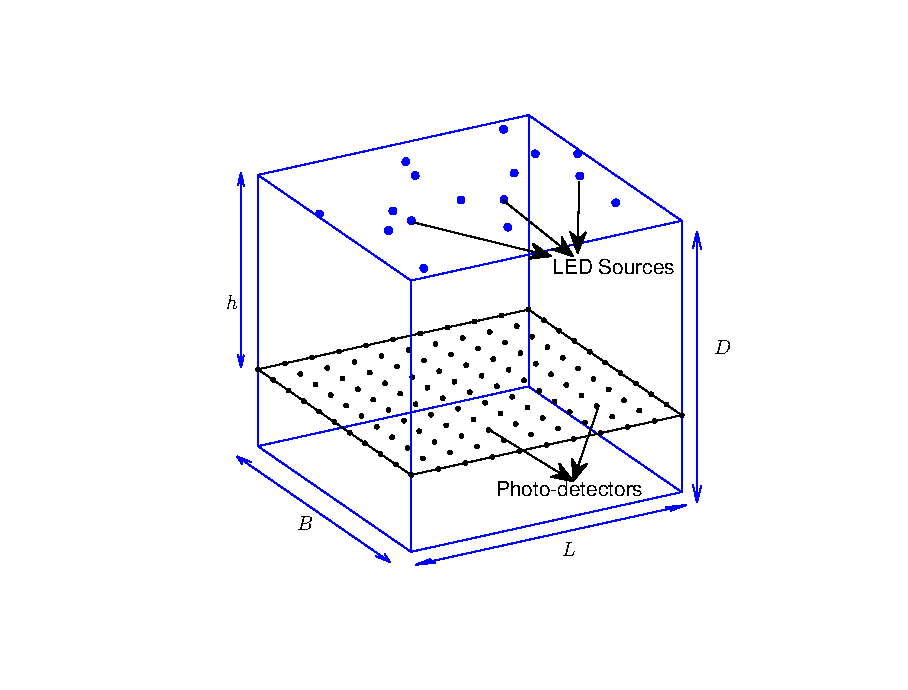
\includegraphics[width=.75\columnwidth]{3dmodel}
\caption{System model}
\label{fig:3dmodel}
\end{figure}
\vfill
\end{frame}

\begin{frame}
\tikzstyle{startstop} = [rectangle, rounded corners, minimum width=2cm, minimum height=.5cm,text centered, draw=black]
\tikzstyle{io} = [trapezium, trapezium left angle=70, trapezium right angle=110, minimum width=3cm, minimum height=.5cm, text centered,text width=3cm, draw=black]
\tikzstyle{process} = [rectangle, minimum width=2cm, minimum height=.5cm, text centered,text width=3.5cm, draw=black]
\tikzstyle{processleft} = [rectangle, minimum width=2cm, minimum height=.5cm, text centered,text width=2.5cm, draw=black]
\tikzstyle{decision} = [diamond, draw, text width=7em, text badly centered,inner sep=0pt]
\tikzstyle{arrow} = [thick,->,>=stealth]
\tikzstyle{line} = [draw,->,>=stealth, -latex']

% ...
%
\begin{figure}[h!]
%\begin{adjustbox}{width=\textwidth,height=\textheight,keepaspectratio}
%\centering
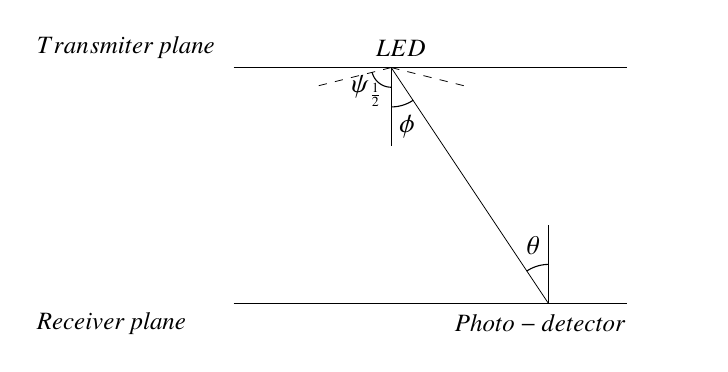
\begin{tikzpicture}[node distance=2cm]

<TikZ code>
\draw[line width=.1mm](-2,3) -- (3,3);
\draw[line width=.1mm](-2,0) -- (3,0);
\draw[line width=.1mm](0,3) -- (2,0);
\draw[line width=.1mm](0,3) -- (0,2);
\draw[line width=.1mm](2,1) -- (2,0);

\draw[dashed,line width=.1mm](0,3) -- (1,2.75);
\draw[dashed,line width=.1mm](0,3) -- (-1,2.75);
\draw [domain=194:270] plot ({0+.25*cos(\x)}, {3+.25*sin(\x)});
\node[] at (-.3,2.7) 
    {$\psi_{\frac{1}{2}}$};
 \draw [domain=90:124] plot ({2+.5*cos(\x)}, {.5*sin(\x)});
  \draw [domain=-90:-56] plot ({.5*cos(\x)}, {3+.5*sin(\x)});
  \node[] at (1.8,.74) 
    {$\theta$};
    \node[] at (.2,2.25) 
    {$\phi$};
    \node[text width=3cm] at (2.3,-.25) 
    {\small $Photo-detector$};
    \node[text width=3cm] at (1.3,3.25) 
    {\small $ LED$};
    \node[text width=3cm] at (-3,-.25) 
    {\small $Receiver \,plane$};
    \node[text width=3cm] at (-3,3.25) 
    {\small $ Transmiter\, plane$};
%\draw(0,2) -- (.5,1);
% \draw[line width=.1mm,red](-1,1.5)--(1,-1.5);
%\draw(-4,-2 -- (4,-2);
% \line(-1,2)(1,2);
\end{tikzpicture}
%\end{adjustbox}
\caption{Propagation model}
\label{fig:algo}
\end{figure}
\end{frame}

\begin{frame}
\frametitle{Introduction}
\framesubtitle{Literature}
\begin{itemize}
\vfill
\item<1->Using the Lambertian radiation pattern to model the LED radiant intensity, %\cite{wireless_infra,funda_vlc}
\begin{equation}
\mathcal{R}\brak{\phi}=\frac{\brak{m+1}\cos^m\brak{\phi}}{2\pi}, \nonumber
\end{equation}
$m=\frac{\ln{\frac{1}{2}}}{\ln\brak{\cos\brak{\psi_{\frac{1}{2}}}}}$ is the order of Lambertian emission, with $\psi_{\frac{1}{2}}$ being the LED semi-angle at half power, provided by the manufacturer.\\
\vfill
\item<2>The channel direct current (DC) gain can then be  expressed as %\cite{wireless_infra,funda_vlc}
\begin{equation}
\label{propagation_old}
H=\frac{\mathcal{R}(\phi)\cos(\theta)A}{d^2}=\frac{\brak{m+1}\cos^m\brak{\phi}A\cos(\theta)}{2\pi d^2} \nonumber
\end{equation}
\vfill
\end{itemize}
\end{frame}


\begin{frame}
\frametitle{Introduction}
\framesubtitle{Literature}
\begin{list}{} {} 
\item<1-> The electrical signal at the output
of the photodetector can be expressed as 
%
\begin{align}
\label{rx_j}
y_j=RP_{r_j}+n_j,\nonumber
\end{align}
%
\item<2->
 where the received optical power at the photodetector $j$
\begin{equation}
P_{r_j} = \sum_{i=1}^NH_{ij}  P_{t_i},\nonumber
\end{equation}
\item<3>
where,
\begin{equation}
\label{propagation}
H_{ij}=\frac{\brak{m+1}Ah^{m+1}}{2\pi d_{ij}^{m+3}}\nonumber
\end{equation}
and $n_j$  is  additive white Gaussian noise (AWGN) with $n_{j}\sim \mathcal{N}\brak{0,\sigma_j^2}$.
\end{list}
\end{frame}

\begin{frame}
\frametitle{Introduction}
\framesubtitle{Literature}
\begin{list}{} {}
\vfill
\item<1->The AWGN noise $n_j$ at the photo-detector is 
the sum of the contributions from shot noise and thermal noise, and expressed as %\cite{berInterfereVLC}
%
\begin{equation}
\label{variance}
\sigma_j^2 = \sigma_{shot}^2+\sigma_{thermal}^2\nonumber
\end{equation}
\vfill
\item<2>where
\begin{equation}
\begin{split}
\sigma_{shot}^2 &= 2qRP_{r_j}B + 2q I_{bg} I_2 B \\
\sigma_{thermal}^2 &=\frac{8\pi kT_k}{G}\eta AI_2B^2 + \frac{16\pi^2kT_k\Gamma}{g_m}\eta^2 A^2I_3B^3
\end{split}\nonumber
\end{equation}
\vfill
\end{list}
\end{frame}
%
\begin{frame}
\frametitle{Introduction}
\framesubtitle{Literature}

\begin{list}{} {}
\vfill
\item<1-> Signal to Noise Ratio (SNR) at photo-detector $j$ is defined as
\begin{equation}
\label{eq:snr}
\Lambda_j = \frac{\brak{RP_{r_j}}^2}{\sigma_j^2}  \nonumber
\end{equation}
\vfill
\item<2-> The quality factor, for measuring the performance  of the light source, can be expressed as
\begin{equation}
\label{quality}
F_{\Lambda}=\frac{\overline{\Lambda}}{2\sqrt{\text{var}(\Lambda)}}, \nonumber
\end{equation}
where 
  $\overline{\Lambda}$  and $\text{var}(\Lambda)$  are the mean and variance of $\cbrak{\Lambda_j}_{j=1}^{K}$, where $K$ is the number of photodetectors. 
\vfill
\end{list}
\end{frame}

\begin{frame}
\frametitle{Introduction}
\framesubtitle{Literature}
\begin{figure}[t!]
    \centering
    \begin{subfigure}[t]{0.4\columnwidth}
        \centering
        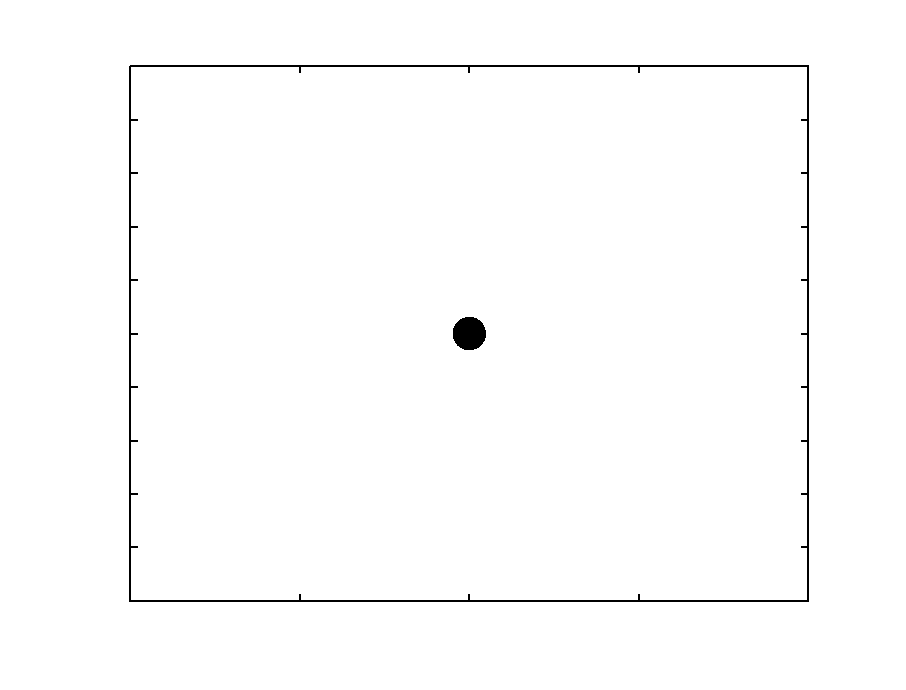
\includegraphics[width=\columnwidth]{point_source}
        \caption{Single point source}
\label{fig3:subfig1}        
    \end{subfigure}%
    ~ 
    \begin{subfigure}[t]{0.4\columnwidth}
        \centering
        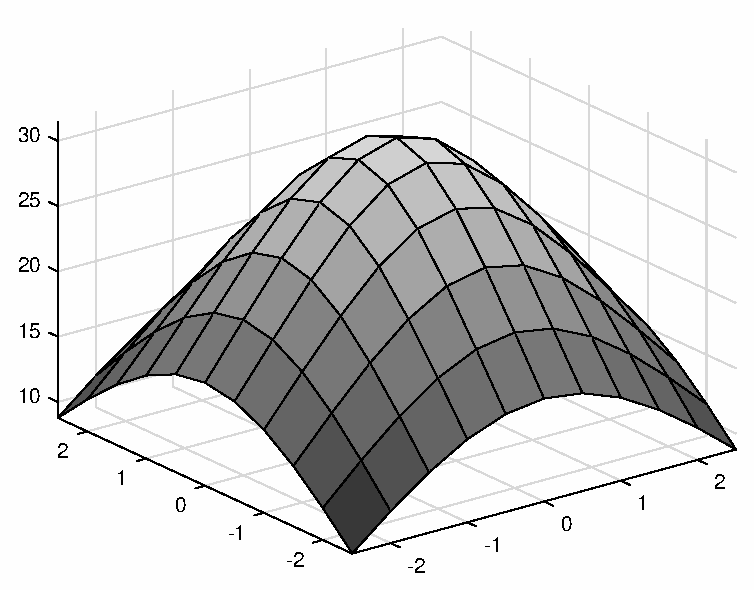
\includegraphics[width=\columnwidth]{pointNoPowerDist_new}
        \caption{SNR profile}
\label{fig3:subfig2}
    \end{subfigure}
  %  \caption{Average SNR for a BPP. $N=16$}
    \label{fig3}
  \end{figure}

\end{frame}
  


%
\subsection{Motivation}
\begin{frame}
\frametitle{Introduction}
\framesubtitle{Motivation}
\begin{figure}
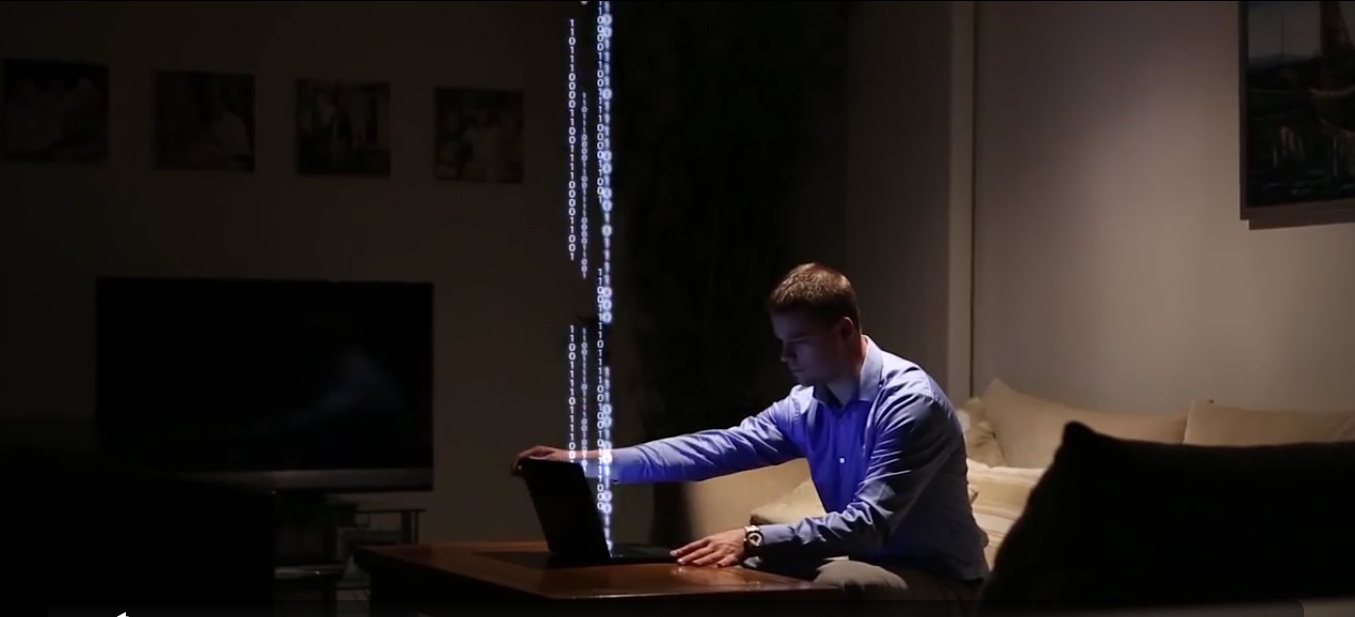
\includegraphics[width=\columnwidth]{point_example}
\end{figure}
\end{frame}

\begin{frame}
\frametitle{Introduction}
\framesubtitle{Motivation}
\begin{figure}[h!]
    \centering
    \begin{subfigure}[t]{0.5\columnwidth}
        \centering
        %\includegraphics[width=\columnwidth]{LedArrangementPoint}
         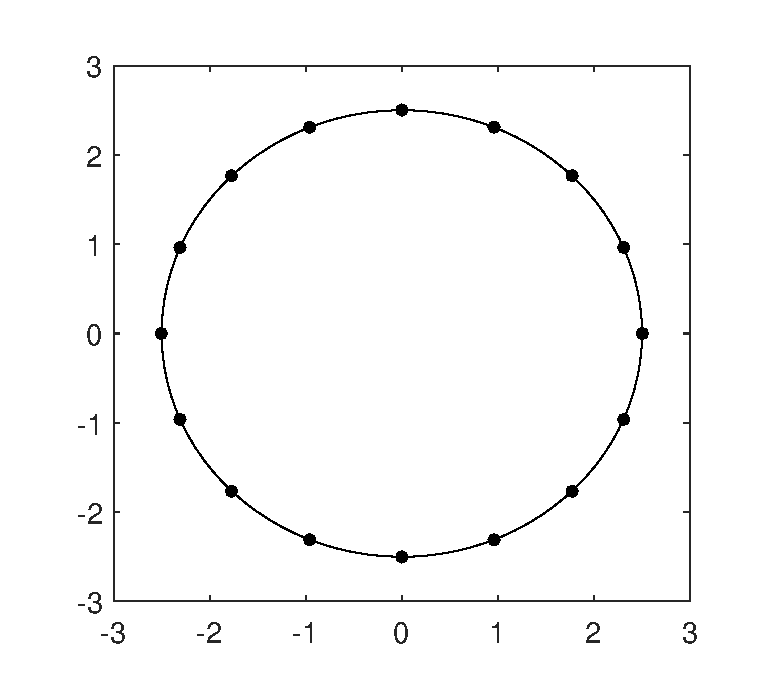
\includegraphics[scale=.25]{LedArrangementCircle}
        \caption{Circular geometry}
\label{fig1:subfig1}        
    \end{subfigure}%
    ~ 
    \begin{subfigure}[t]{0.5\columnwidth}
        \centering
        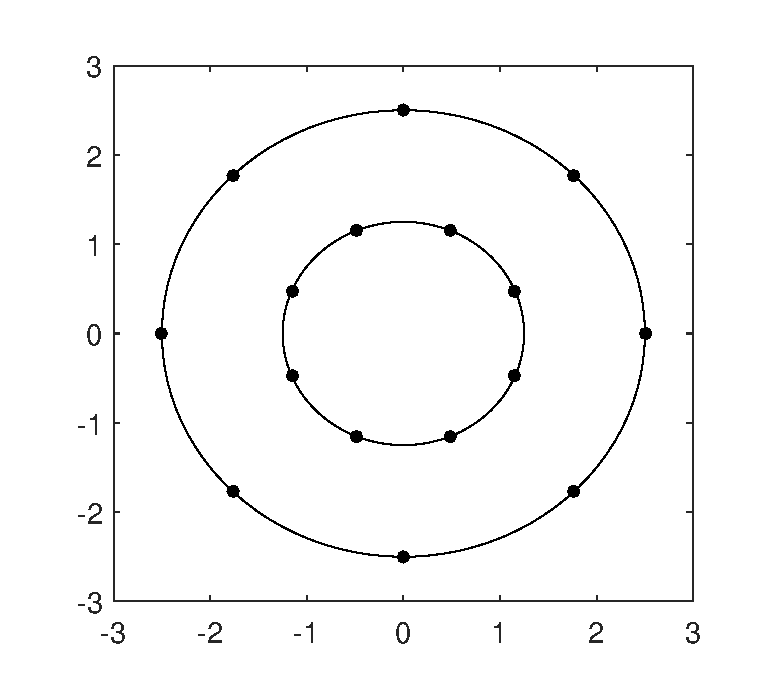
\includegraphics[scale=.25]{LedArrangementConcircle}
        \caption{Concentric circular geometry}
\label{fig1:subfig2}
    \end{subfigure}

    \begin{subfigure}[t]{0.5\columnwidth}
        \centering
        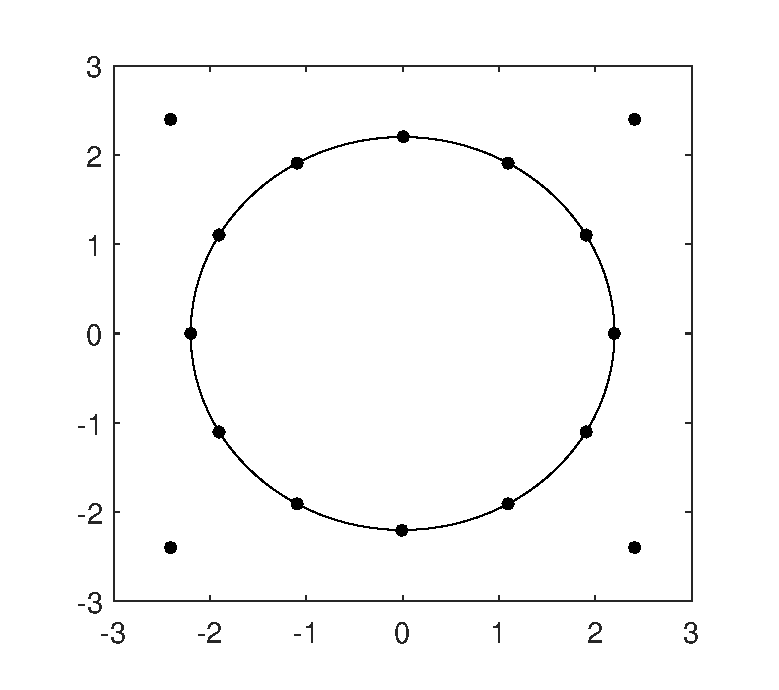
\includegraphics[scale=.25]{LedArrangementPaper}
        \caption{Circle-square geometry }
\label{fig1:subfig4}
    \end{subfigure}
       \caption{Arrangement of LEDs for different geometries}
    \label{geometries}
\end{figure}
\end{frame}

\begin{frame}
\frametitle{Introduction}
\framesubtitle{Motivation}

\begin{figure}[h!]
    \centering

    \begin{subfigure}[t]{.5\columnwidth}
        \centering
        %\includegraphics[width=\columnwidth]{LedArrangementPoint}
         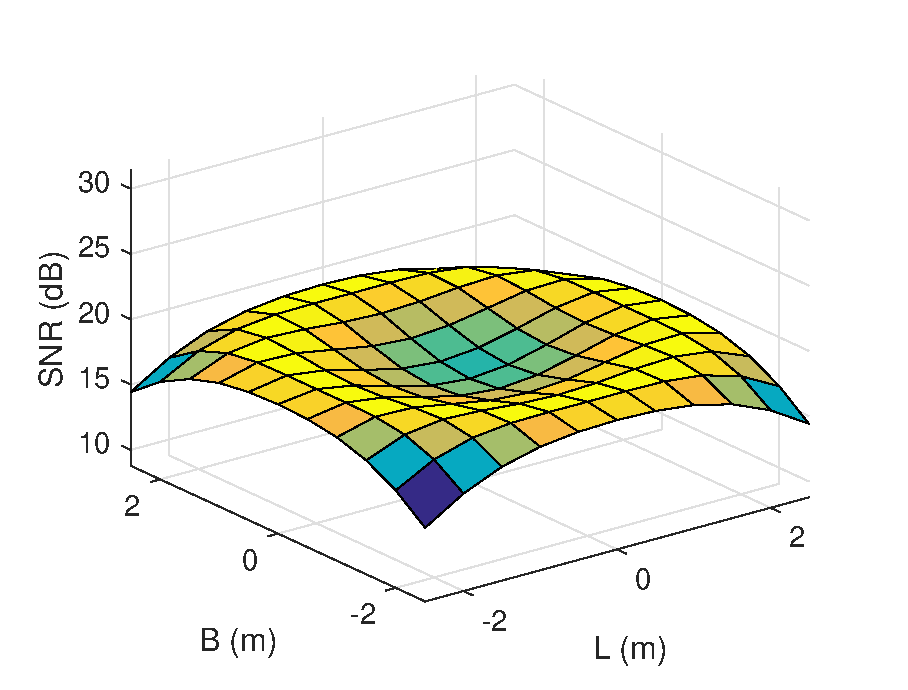
\includegraphics[width=\columnwidth]{circleNoPowerDist_new}
        \caption{Circular geometry}
\label{fig2:subfig1}        
    \end{subfigure}%
    ~ 
    \begin{subfigure}[t]{.5\columnwidth}
        \centering
        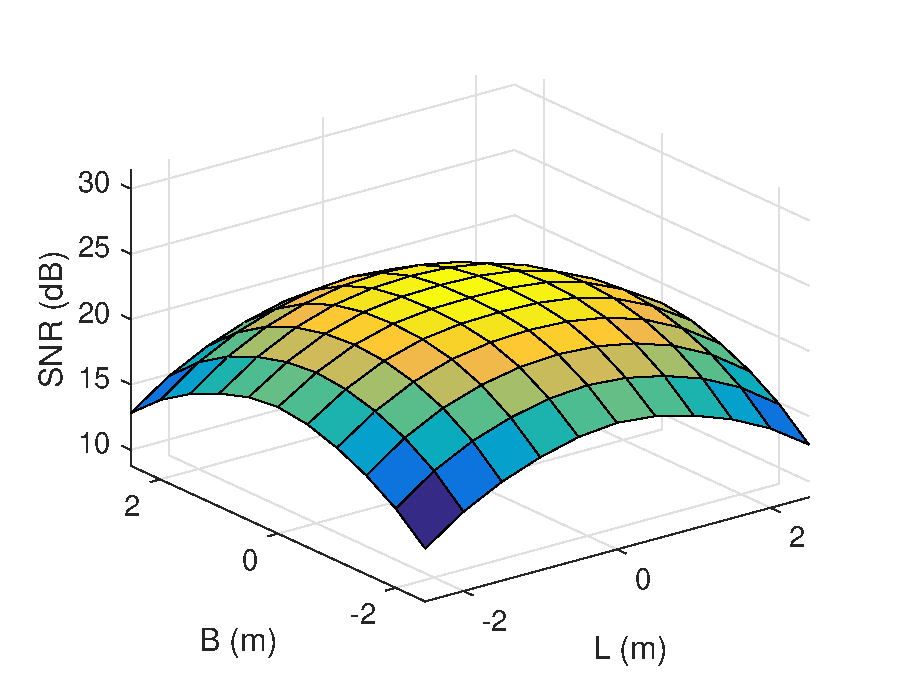
\includegraphics[width=\columnwidth]{concircleNoPowerDist_new}
        \caption{Concentric Circular }
\label{fig2:subfig2}
    \end{subfigure}
    \caption{SNR distribution with equal power allocation}
    \label{fig:SNRDistCircles}
    \end{figure}
\end{frame}

    
    \begin{frame}
\frametitle{Introduction}
\framesubtitle{Motivation}
\begin{figure}[h!]
    \centering
         \begin{subfigure}[t]{0.48\columnwidth}
        \centering
        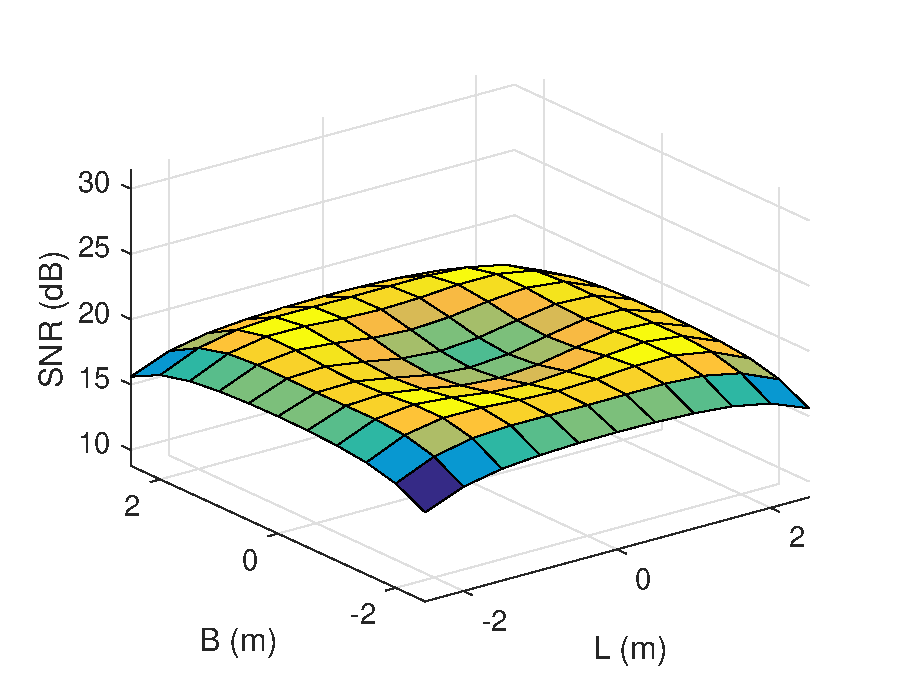
\includegraphics[width=\columnwidth]{cirsqNoPowerDist_new}
        \caption{With equal power allocation and optimal location}
\label{fig2:subfig3}     
    \end{subfigure}%
~ 
    \begin{subfigure}[t]{0.48\columnwidth}
        \centering
        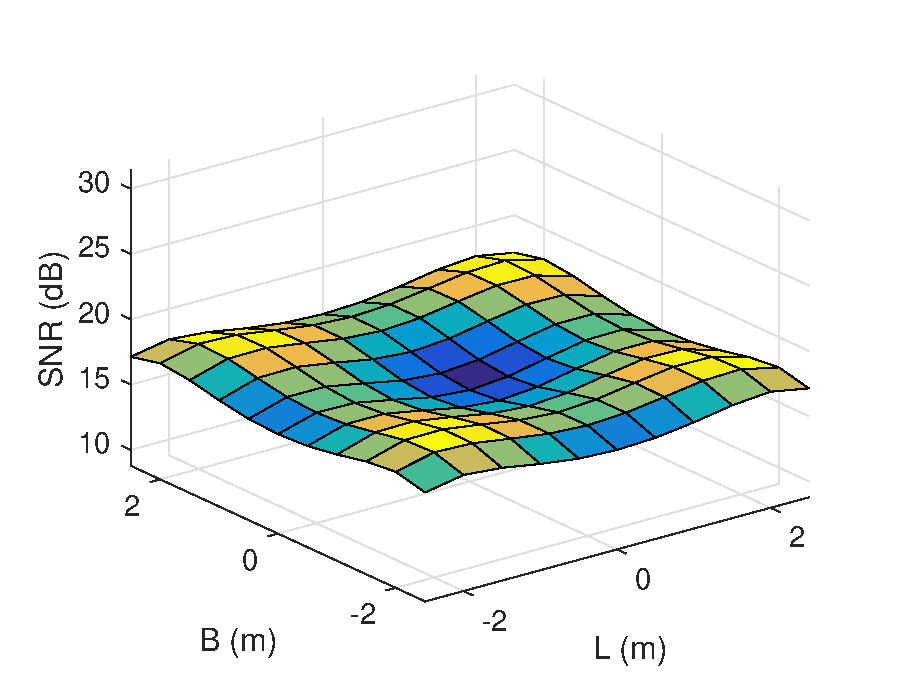
\includegraphics[width=\columnwidth]{cirsqPowerDist_new}
        \caption{With optimal power allocation and optimal location}
\label{fig2:subfig4}
    \end{subfigure}
    \caption{SNR distribution for circle-square geometry}
    \label{fig:SNRDistCirsq}
\end{figure}
\end{frame}

\section{Problems Addressed}
\subsection{Power Allocation for Uniform Illumination with Stochastic LED Arrays}

\begin{frame}
\vfill
Power Allocation for Uniform Illumination with Stochastic LED Arrays
\vfill
\end{frame}
\begin{frame}
\frametitle{\,}
\framesubtitle{Power Allocation for Uniform Illumination with
Stochastic LED Arrays}
\begin{figure}[t!]
    \centering
    \begin{subfigure}[t]{0.5\columnwidth}
        \centering
        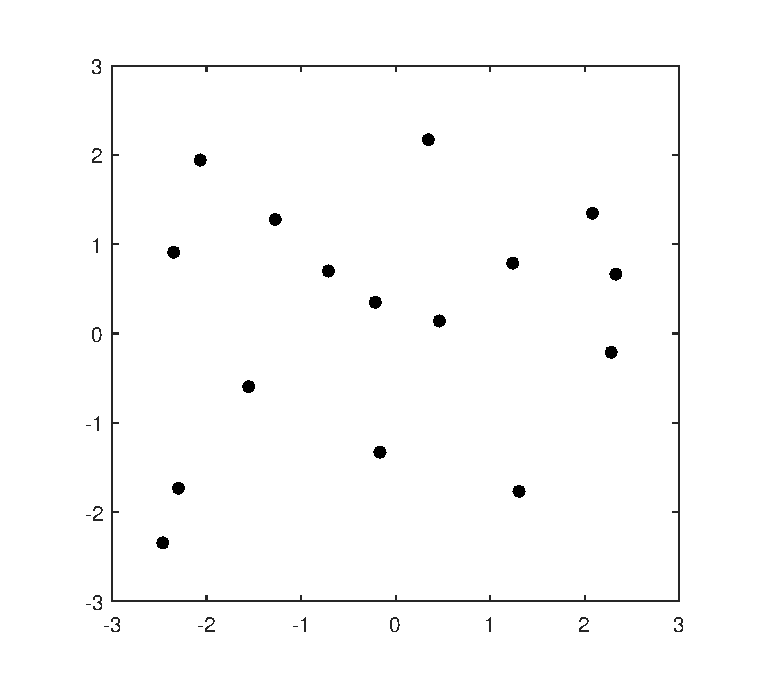
\includegraphics[width=\columnwidth]{LedArrangementRandom}
        \caption{A realization of BPP}
\label{fig3:subfig1}        
    \end{subfigure}%
    ~ 
    \begin{subfigure}[t]{0.5\columnwidth}
        \centering
        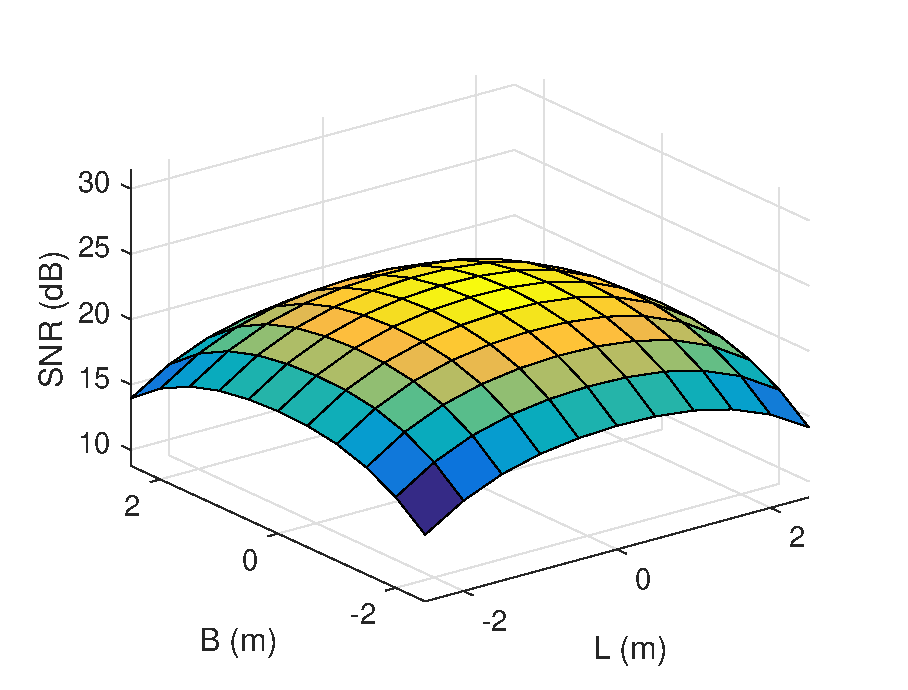
\includegraphics[width=\columnwidth]{randomNoPowerDist_new}
        \caption{Average SNR profile with equal power allocation}
\label{fig3:subfig2}
    \end{subfigure}
  \end{figure}
\end{frame}

%\begin{frame}
%\frametitle{Problems Addressed}
%\framesubtitle{Power Allocation for Uniform Illumination with
%Stochastic LED Arrays}
%\begin{table}
%\begin{tabular}{|c|c|c|}
%\hline
%$P_{center}$&$P_{corner}$ &$\sum \frac{1}{d_{ij}^a} \sum\frac{1}{r_{ij}^a}$
%\hline
%$\sbrak{0,\frac{L}{\sqrt{2}}}$& $\sbrak{0,\sqrt{2}L}$&
%\end{tabular}
%\end{table}
%\end{frame}

\begin{frame}
\frametitle{\,}
\framesubtitle{Power Allocation for Uniform Illumination with
Stochastic LED Arrays}
\begin{list}{}{}
\item \textcolor{blue}{Heuristic power allocation:}
\begin{align}
\label{power_alloc}
P_{t_i}=\frac{r_i^{\alpha}}{\sum_{n=1}^Nr_n^{\alpha}}P,\nonumber
\end{align}
\end{list}
 \end{frame}


\begin{frame}
\frametitle{\,}
\framesubtitle{Power Allocation for Uniform Illumination with
Stochastic LED Arrays}
   \begin{figure}[!h]
        \centering
        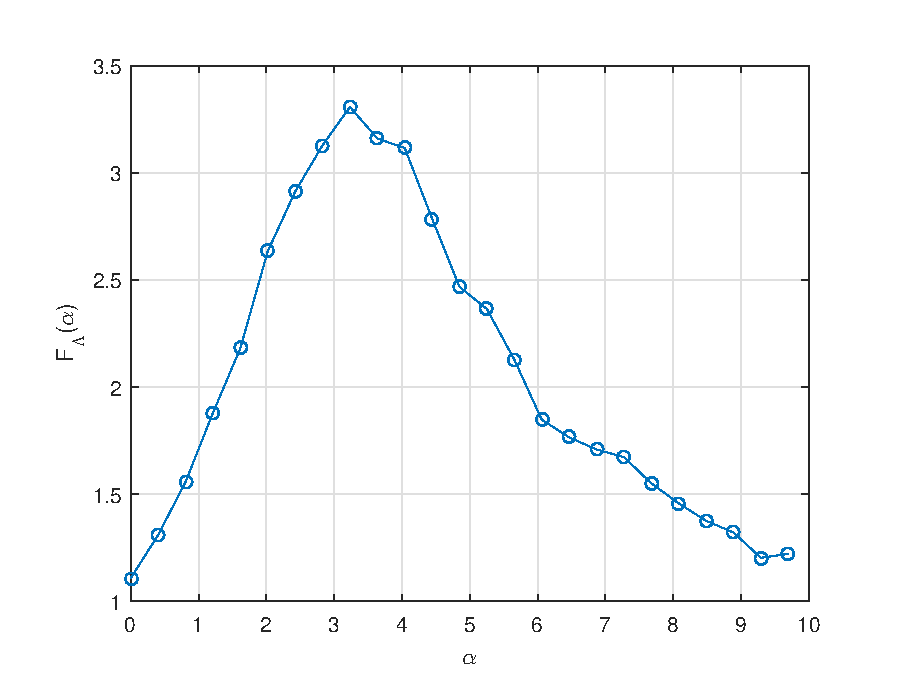
\includegraphics[width=.6\columnwidth]{QvsAlpha}
        \caption{$F_{\Lambda}(\alpha)$ has a maximum.}
	\label{fig:qconcave}
    \end{figure}
    \textcolor{blue}{Optimum value of $\alpha$ is obtained from golden section search algorithm}
\end{frame}

\begin{frame}
\frametitle{\,}
\framesubtitle{Power Allocation for Uniform Illumination with
Stochastic LED Arrays}
\begin{figure}[t!]
    \centering
    \begin{subfigure}[t]{0.5\columnwidth}
        \centering
        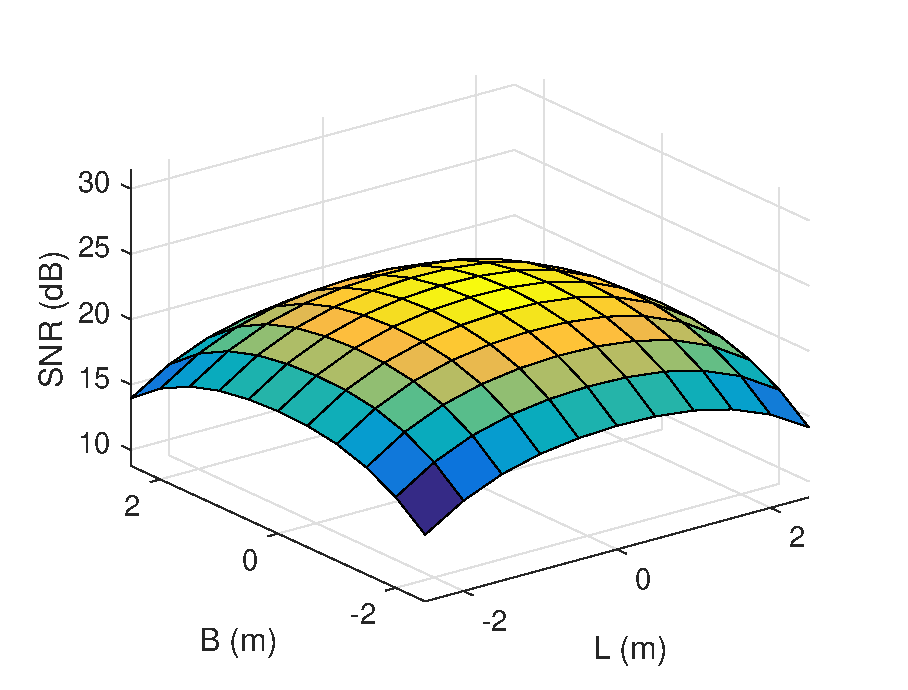
\includegraphics[width=\columnwidth]{randomNoPowerDist_new}
        \caption{Equal power allocation}
\label{fig3:subfig1}        
    \end{subfigure}%
    ~ 
    \begin{subfigure}[t]{0.5\columnwidth}
        \centering
        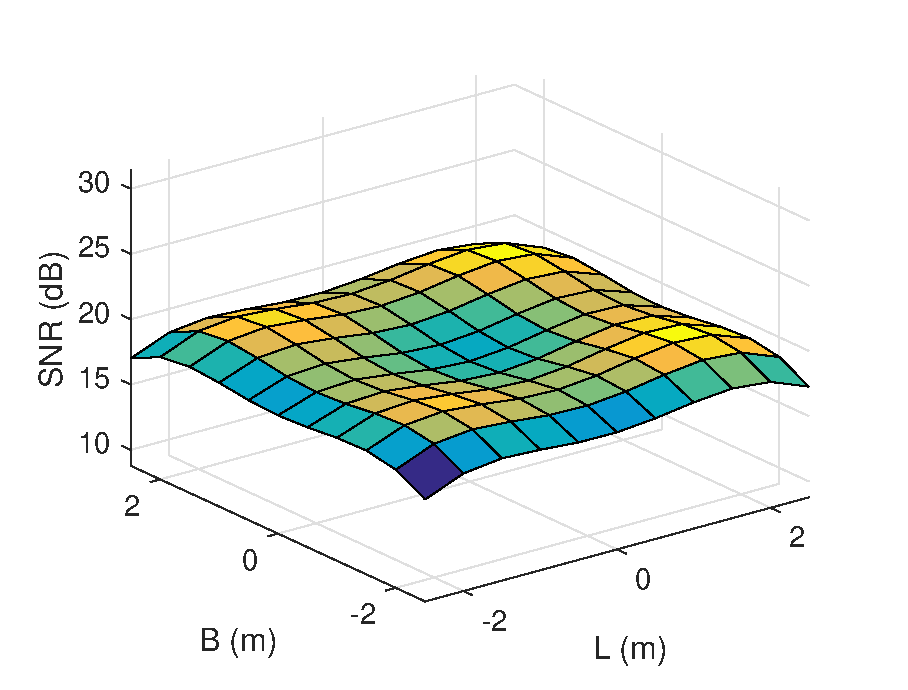
\includegraphics[width=\columnwidth]{randomPowerDist_new}
        \caption{Suboptimal power allocation}
\label{fig3:subfig2}
    \end{subfigure}
    \caption{Average SNR for a BPP. $N=16$}
    \label{fig3}
  \end{figure}  
\end{frame}

\begin{frame}
\frametitle{\,}
\framesubtitle{Power Allocation for Uniform Illumination with
Stochastic LED Arrays}
\begin{figure}[h!]
    \centering
    \begin{subfigure}[t]{0.5\columnwidth}
        \centering
        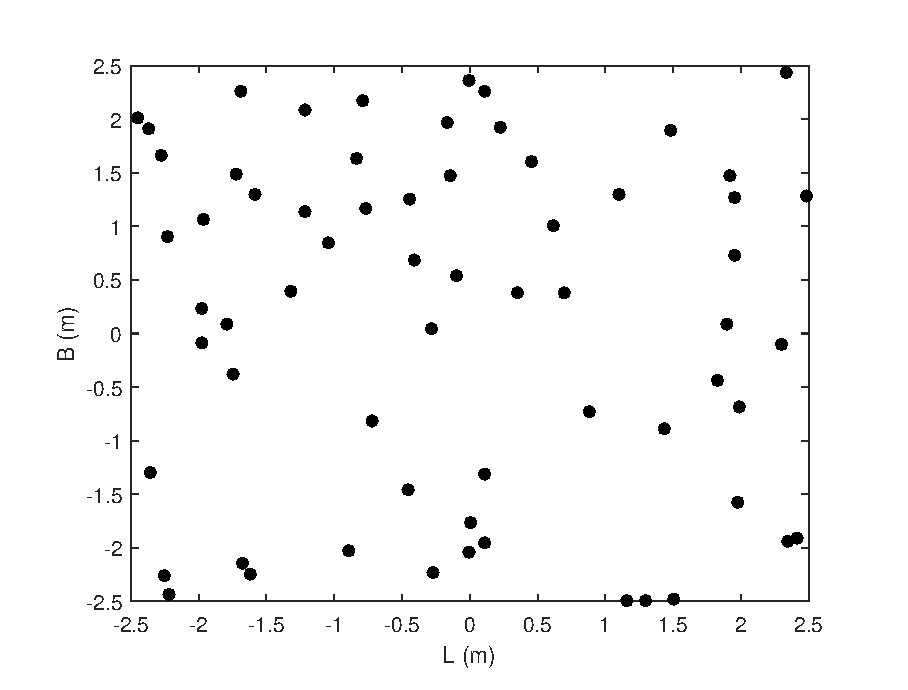
\includegraphics[scale=.2]{LEDRealization1}
        \caption{$N=64$, BPP realization 1}
\label{fig:two_realize:led1}        
    \end{subfigure}%
    ~ 
    \begin{subfigure}[t]{0.5\columnwidth}
        \centering
        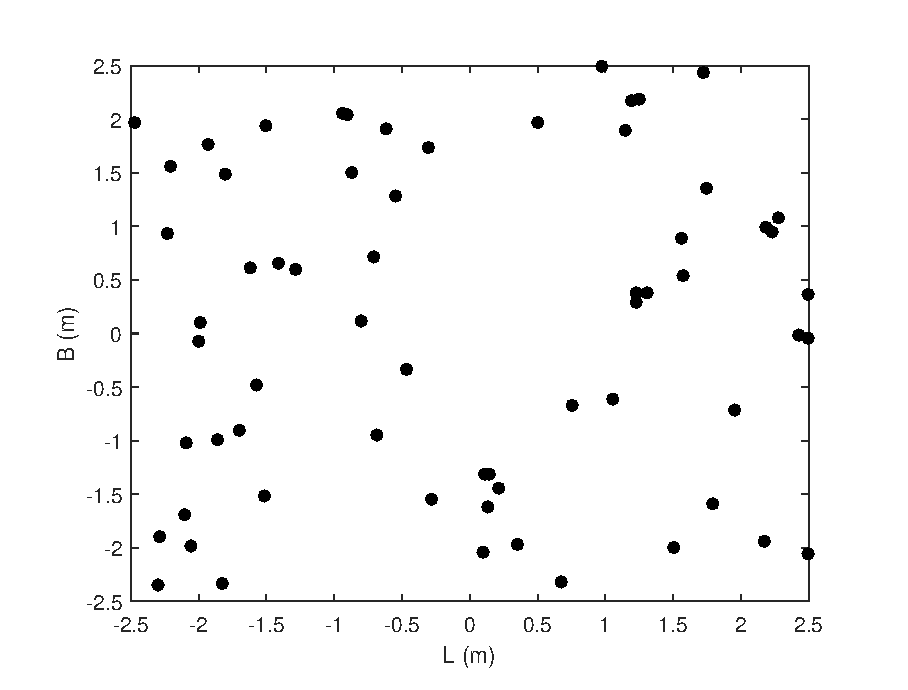
\includegraphics[scale=.2]{LEDRealization2}
        \caption{$N=64$, BPP realization 2}
\label{fig:two_realize:led2}
    \end{subfigure}
        \begin{subfigure}[t]{0.5\columnwidth}
        \centering
        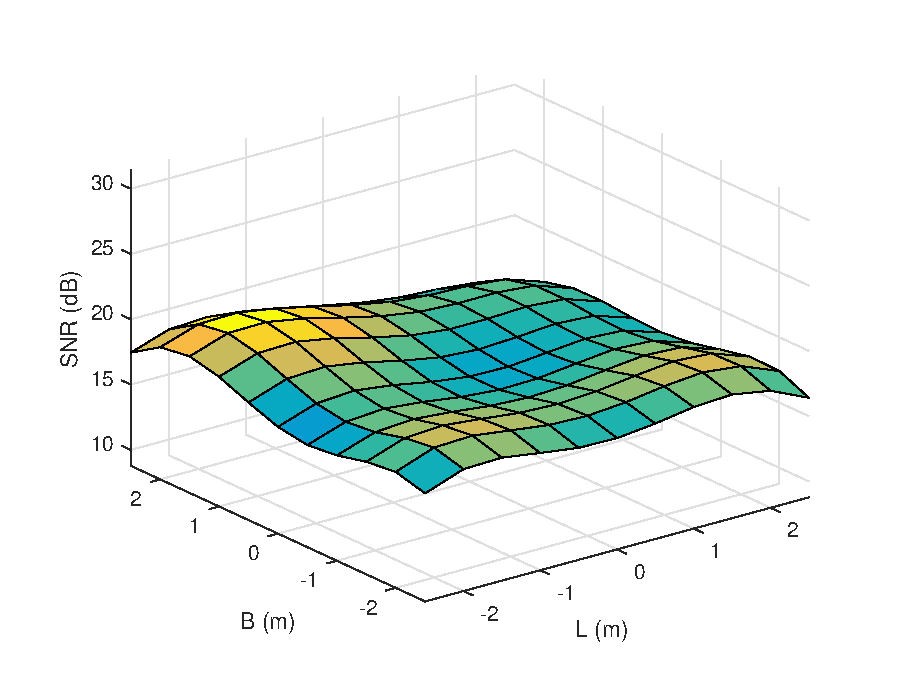
\includegraphics[scale=.2]{snrRealization1}
        \caption{SNR profile for realization 1}
\label{fig:two_realize:snr1}        
    \end{subfigure}%
    ~ 
    \begin{subfigure}[t]{0.5\columnwidth}
        \centering
        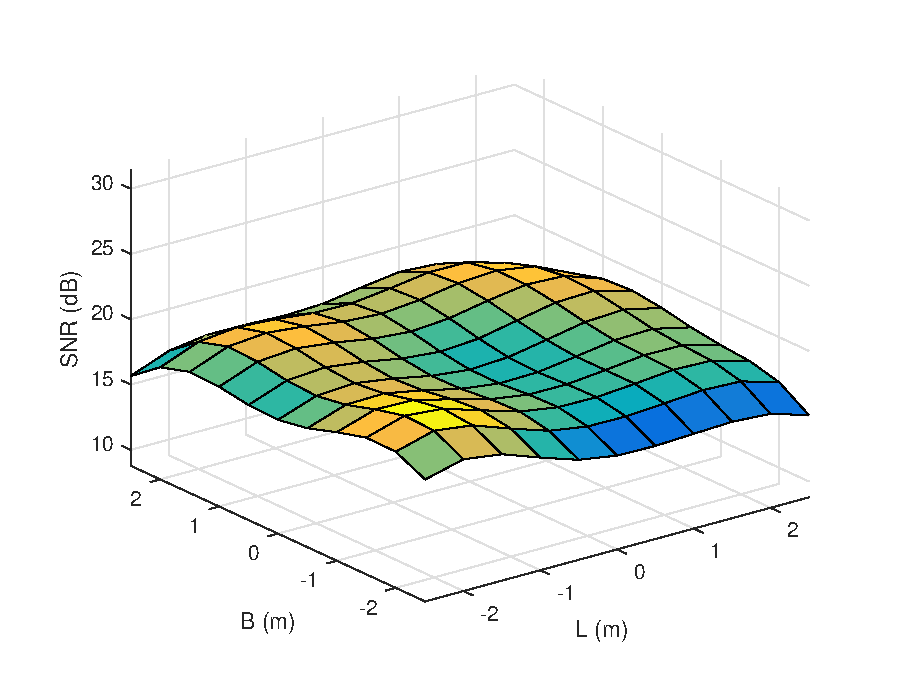
\includegraphics[scale=.2]{snrRealization2}
        \caption{SNR profile for realization 2}
\label{fig:two_realize:snr2}
    \end{subfigure}

   % \caption{SNR for two different realizations for $N=64$.  }
    \label{fig:two_realize}
  \end{figure}  
  \begin{list}{}{}
 \item \textcolor{blue}{Uniform illumination possible with random distribution.}
  \end{list}
\end{frame}



\subsection{Performance of Stochastic LED Arrays based VLC}
\begin{frame}
\vfill
Performance of Stochastic LED Arrays based VLC with Uniform Irradiance
\vfill
\end{frame}
\begin{frame}
\frametitle{\,}
\framesubtitle{Performance of Stochastic LED Arrays based VLC with Uniform Irradiance}
   \begin{figure}
        \centering
        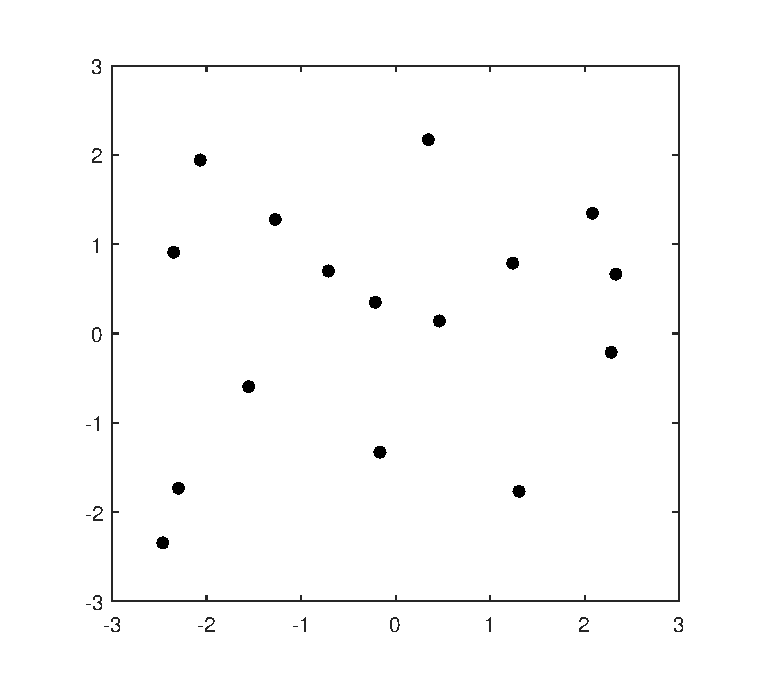
\includegraphics[width=.6\framewidth]{LedArrangementRandom}
        \caption{Realization of a BPP}
        \end{figure}
\end{frame}

\begin{frame}
\frametitle{\,}
\framesubtitle{Performance of Stochastic LED Arrays based VLC with Uniform Irradiance}
\begin{list}{}{}
\vfill
\item<1->The optical signal transmitted by the $i$th LED of a VLC is given by %\cite{novel_led}
%
\begin{equation}
p_i(t) = P_{t_i} \sbrak{1 + M_I x_i(t)},\nonumber
\end{equation}
\vfill
\item<2>After removing DC component, the signal received at $j$th photo-detector from all the source LEDs is 
\begin{align}
\label{rx_j}
y_j=RP_{r_j}+n_j\nonumber
\end{align}

\vfill
where,
\begin{equation}
\label{rx_pow}
P_{r_j}=\sum_{i=1}^NH_{ij}P_{t_i}M_Ix_i.\nonumber
\end{equation}
\vfill
\end{list}
\end{frame}
%
\begin{frame}
\frametitle{\,}
\framesubtitle{Performance of Stochastic LED Arrays based VLC with Uniform Irradiance}
\begin{list}{}{}
\vfill
\item<1->The AWGN noise $n_j$ at the photo-detector is 
the sum of the contributions from shot noise and thermal noise, and expressed as %\cite{berInterfereVLC}
%
\begin{equation}
\label{variance}
\sigma_j^2 = \sigma_{shot}^2+\sigma_{thermal}^2 \nonumber
\end{equation}
\vfill
where
\begin{equation}
\begin{split}
\sigma_{shot}^2 &= 2qRP_{r_j}B + 2q I_{bg} I_2 B \\
\sigma_{thermal}^2 &=\frac{8\pi kT_k}{G}\eta AI_2B^2 + \frac{16\pi^2kT_k\Gamma}{g_m}\eta^2 A^2I_3B^3
\end{split}\nonumber
\end{equation}
\vfill
\item<2> \textcolor{blue}{Heuristic power allocation:}\\
The transmit power at the $i$th transmitter is 
given by the heuristic
\begin{align}
\label{power_alloc}
P_{t_i}=\frac{r_i^{\alpha}}{\sum_{j=1}^Nr_j^{\alpha}}P,\nonumber
\end{align}
\vfill
\end{list}
\end{frame}


\begin{frame}
\frametitle{\,}
\framesubtitle{Performance of Stochastic LED Arrays based VLC with Uniform Irradiance}
\begin{list}{}{}
\vfill
\item<1->The received symbol at the central photodetector is given by 
\begin{equation}
y=RP_{r_0}+n_0 \nonumber
\label{rx_center}
\end{equation}
and,
\item<2>
\vspace{-.4in}
\begin{align}
P_{r_0}
=C_1\sum_{i=1}^NV_i x_i  \nonumber
\label{pr_exact}
\end{align}
where $x_i$ is the modulating bipolar OOK signal. All LEDs are assumed to transmit the same message signal.
\footnotesize{
\begin{equation}
\begin{split}
C_1&=\frac{PM_I\brak{m+1}Ah^{m+1}}{2\pi} \quad \text{and}
\\
V_i &= \frac{r_i^{\alpha}}{ \brak{\sum_{j=1}^Nr_j^{\alpha}}\brak{\sqrt{h^2+r_i^2}}^{m+3}}.
\end{split} \nonumber
\label{variable_Vi}
\end{equation}
}
\vfill
\end{list}
\end{frame}

\begin{frame}
\frametitle{\,}
\framesubtitle{Performance of Stochastic LED Arrays based VLC with Uniform Irradiance}
\begin{list}{}{}
\vfill
\item<1->
\begin{equation}
y =  \brak{RC_1\sum_{i=1}^NV_i}x+n_0 \nonumber
\label{rx_exact}
\end{equation}
\vfill
\item<2->
BER for this system is given by
\begin{equation}
P_e  =\mathbb{E}_{\Phi}\sbrak{\textit{Q}\brak{\frac{RC_1\sum_{i=1}^N V_i}{\sigma_0}}} \nonumber
\end{equation}
\vfill
\item<3>
 Using first order taylor approximation, Schwarz's inequality, and Jensen's inequality the above expresseion is reduced to
\begin{equation}
\begin{split}
P_e  &\gtrapprox  \textit{Q}\brak{\frac{RC_1\sum_{i=1}^N \mathbb{E}_{\Phi}\sbrak {V_i}}{ \sqrt{\mathbb{E}_{\Phi}\sbrak{\sigma_0^2}}}}
  \end{split}\nonumber
\label{BER_final}
\end{equation}
\vfill
\end{list}
\end{frame}

\begin{frame}
\frametitle{\,}
\framesubtitle{Performance of Stochastic LED Arrays based VLC with Uniform Irradiance}

\begin{list}{}{}

\vfill
\item<1->
\footnotesize{
For a BPP distributed over a square region of area $W$,
the probability density function (PDF) of the distance to the $i^{th}$ nearest LED from the origin
is
%
\begin{equation}
f_{r_i}=\begin{cases} 
      \frac{2\pi r}{W}\frac{\brak{1-p}^{N-i}p^{i-1}}{\mathcal{B}\brak{N-i+1,i}} & 0 < r < R_{in}\\
      \frac{2\brak{\pi-4\theta} r}{W}\frac{\brak{1-q}^{N-i}q^{i-1}}{\mathcal{B}\brak{N-i+1,i}} & R_{in} < r < R_c \\
      0 &  R_c < r
   \end{cases}\nonumber
   \end{equation}
 where $\theta=\cos^{-1}\brak{R_{in}/r}$, $p=\frac{\pi r^2}{W}$, $q=\frac{\pi r^2-4r^2\theta+2 r^2\sin\brak{2\theta}}{W}$, $R_{in}$ and $R_c$ are the radii of the incircle and circumcircle of $W$.
 }
 \vfill

 \item<2>
\tiny{
\begin{multline}
\label{e_phi}
\mathbb{E}_{\Phi}\sbrak{V_i}
= \frac{1}{\sum_{j=1}^N\mathbb{E}_{\Phi}\sbrak{r_j^{\alpha}} }\lsbrak{\frac{R_{in}^{\alpha}}{h^{m+3}\mathcal{B}\brak{N-i+1,i}} \times} \\
\sum_{k=0}^{N-i}\frac{\binom{N-i}{k}(-1)^k}{\brak{k+i+\alpha/2}}\brak{\frac{\pi R_{in}^2}{W}}^{k+i}
%   \nonumber \\
%   &\quad \times 
   \,_2F_1\brak{\frac{m+3}{2},k+i+\alpha/2;k+i+\alpha/2+1;-\frac{R_{in}^2}{h^2}} 
\\
\rsbrak{+ \frac{R_{in}^{\alpha}}{\mathcal{B}\brak{N-i+1,i}}\sum_{k=0}^{N-i}\binom{N-i}{k}(-1)^k\brak{\frac{R_{in}^2}{W}}^{k+i}
 %  \nonumber \\
%   &\quad \times 
   \int_{0}^{\frac{\pi}{4}} \frac{}{}
%   \nonumber 
%   \\ & 
%   \qquad \times 
   \frac{2\brak{\pi-4\theta}\sin\brak{\theta}\brak{\pi -4\theta+2\sin\brak{2\theta}}^{k+i-1}}{\cos^{2\brak{k+i-1}+\alpha-m}\brak{\theta}\brak{\sqrt{R_{in}^2+h^2\cos^2\brak{\theta}}}^{m+3}} d \theta  }\nonumber
\end{multline}
}
 \end{list}
 
\end{frame}

\begin{frame}
\frametitle{\,}
\framesubtitle{Performance of Stochastic LED Arrays based VLC with Uniform Irradiance}
\begin{figure}
 \begin{subfigure}[t]{0.49\framewidth}
      \centering
      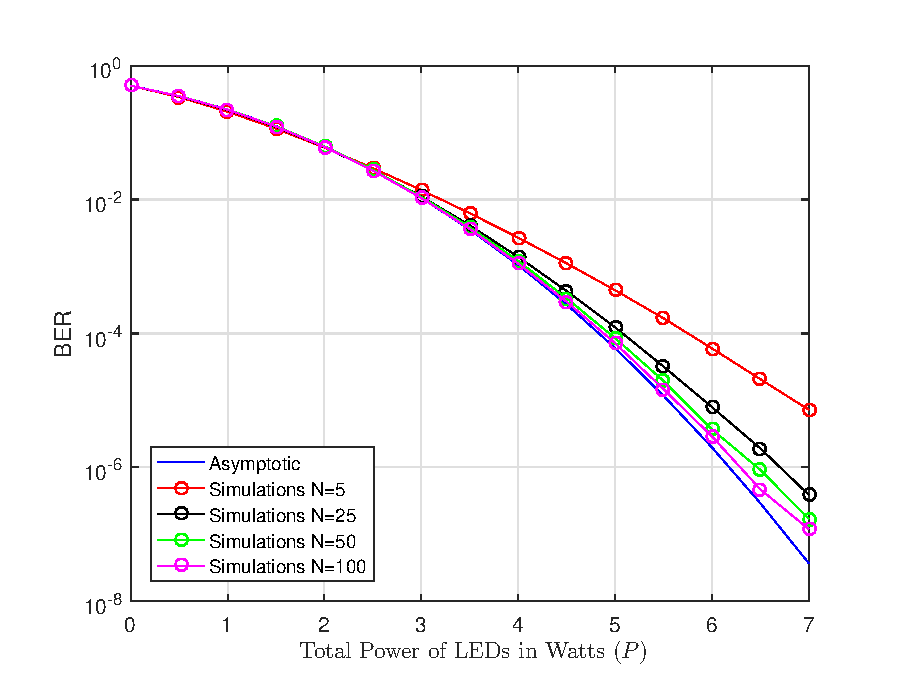
\includegraphics[width=\columnwidth]{berCurveVariousN}
      \caption{ BER performance with respect to source power for different number of LEDs}
            \label{fig:PeVSSnr}
 \end{subfigure} 
 \begin{subfigure}[t]{0.49\framewidth}
      \centering
      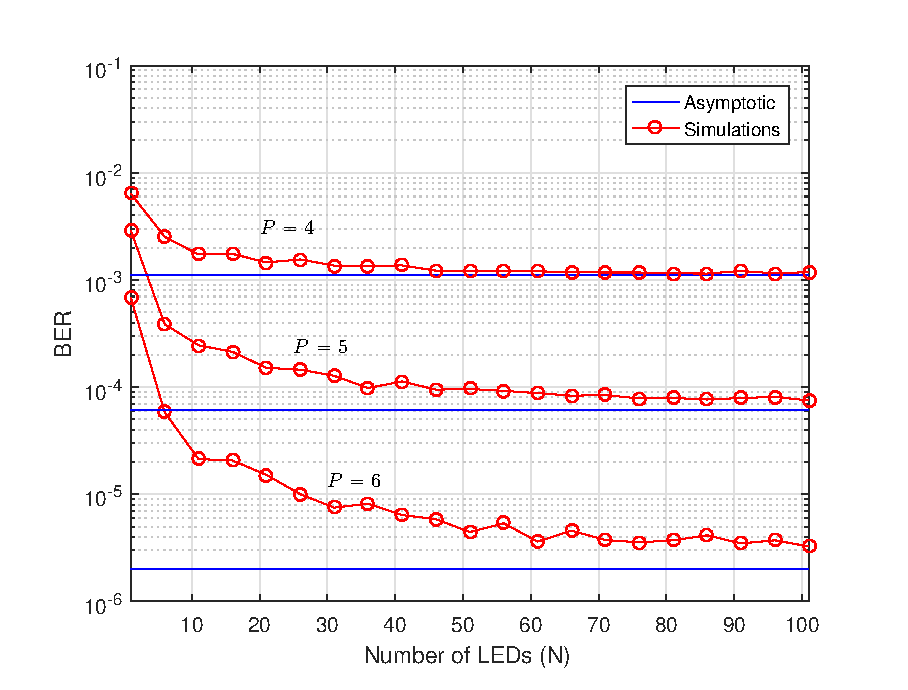
\includegraphics[width=\columnwidth]{berCurveVSN}
      \caption{Convergence of BER with respect to number of LEDs}
         \label{fig:PeConvergence}
 \end{subfigure} 
\end{figure}
\end{frame}

\subsection{Closed-form expressions of BER for BPP in circular region}
\begin{frame}
\vfill
\centering
Closed-form expressions of BER for BPP in circular region
\vfill
\end{frame}
\begin{frame}
\frametitle{\,}
\framesubtitle{Closed-form expressions of BER for BPP in circular region}
\vfill
Source LEDs are distributed uniformly in circular region of radius $R_c$(circumference of dimension of room).
\begin{figure}
        \centering
        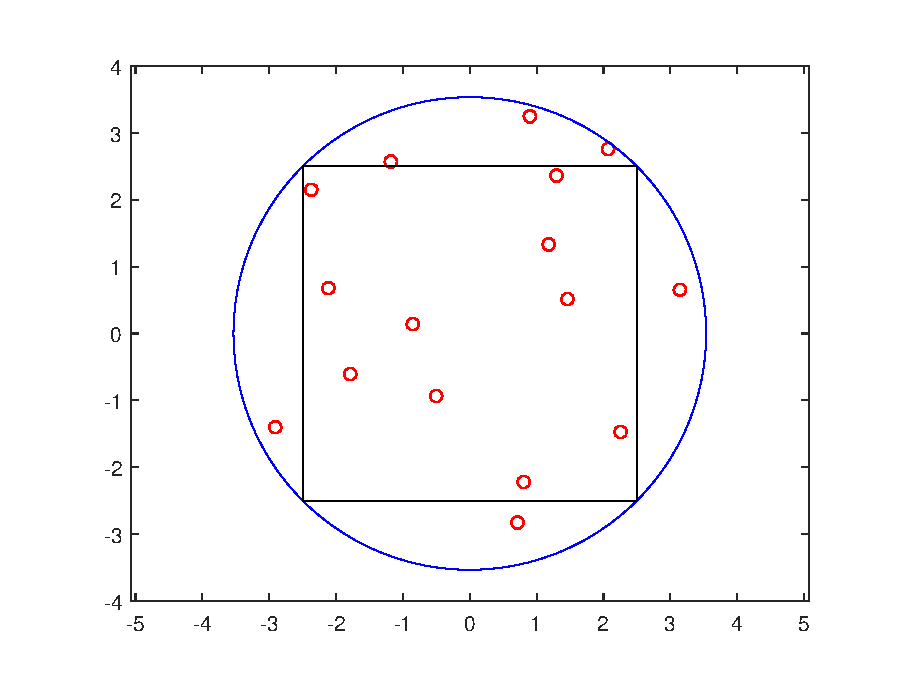
\includegraphics[width=.6\framewidth]{LEDArrangementCircumcircle}
        \caption{Realization of a circular BPP}
        \end{figure}
\end{frame}

\begin{frame}
\frametitle{\,}
\framesubtitle{Closed-form expressions of BER for BPP in circular region}
\begin{list}{}{}
\vfill
\item<1->
The PDF of the distance of $i^{th}$ nearest LED location from origin for circular BPP for $0 \leq r \leq R_c$ is given by %\cite{uniform_distance}
\begin{align}
f_{r_i}	&=
\frac{2r}{R_c^2 B\brak{i,N-i+1}}\brak{\frac{r^2}{R_c^2}}^{i-1}\brak{1-\frac{r^2}{R_c^2}}^{N-i}
\nonumber 
   \end{align}
   \vfill
   \item<2->
   \begin{align}
   \mathbb{E}_{\Phi}\sbrak{r_i^{\alpha}} & =\frac{R_c^{\alpha}}{\mathcal{B}\brak{N-i+1,i}}\sum_{k=0}^{N-i}\frac{\binom{N-i}{k}\brak{-1}^{k}}{\brak{i+k+\frac{\alpha}{2}}}  \nonumber
      \end{align}
      
      \vfill
\item<3>
      \begin{align}
   \mathbb{E}_{\Phi}\sbrak{V_i}
     &=\frac{R_c^{\alpha}}{h^{m+3}\mathcal{B}\brak{N-i+1,i}\sum_{j=1}^N\mathbb{E}_{\Phi}\sbrak{r_j^{\alpha}}} \sum_{k=0}^{N-i}\frac{\binom{N-i}{k}(-1)^{k}}{\brak{i+k+\frac{\alpha}{2}}} \nonumber\\
    & \quad \times  \, _2F_1\brak{\frac{m+3}{2},i+k+\frac{\alpha}{2};i+k+\frac{\alpha}{2}+1;-\frac{R_c^2}{h^2}} \nonumber
   \end{align}
   \vfill
   \end{list}
\end{frame}

\begin{frame}
\frametitle{\,}
\framesubtitle{Closed-form expressions of BER for BPP in circular region}
\begin{figure}
 \begin{subfigure}[t]{0.49\framewidth}
        \centering
        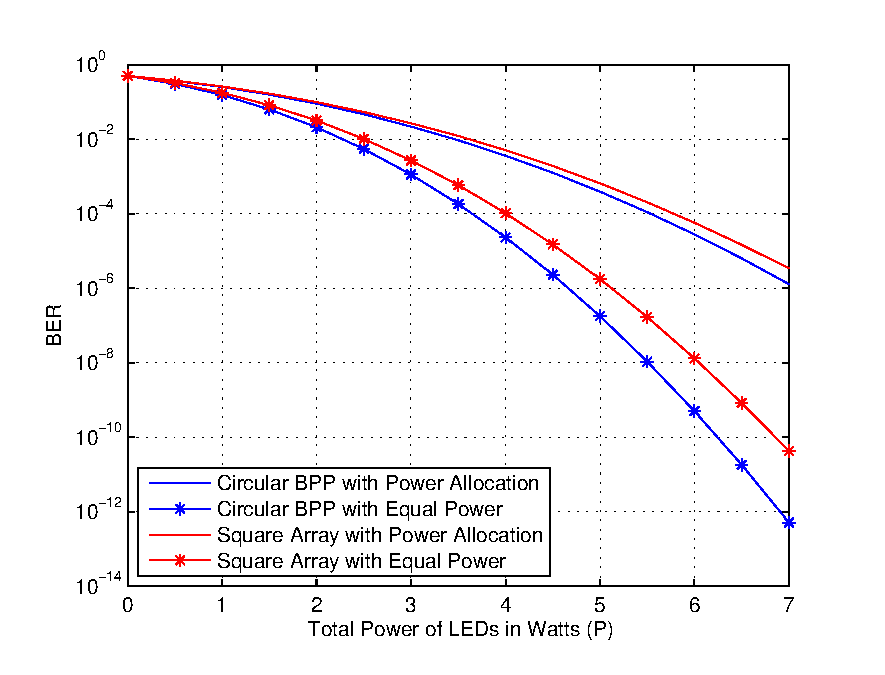
\includegraphics[width=\columnwidth]{berVSp}
      %  \caption{Circular BPP}
\label{fig1:subfig4}
    \end{subfigure}
        \begin{subfigure}[t]{0.49\framewidth}
        \centering
        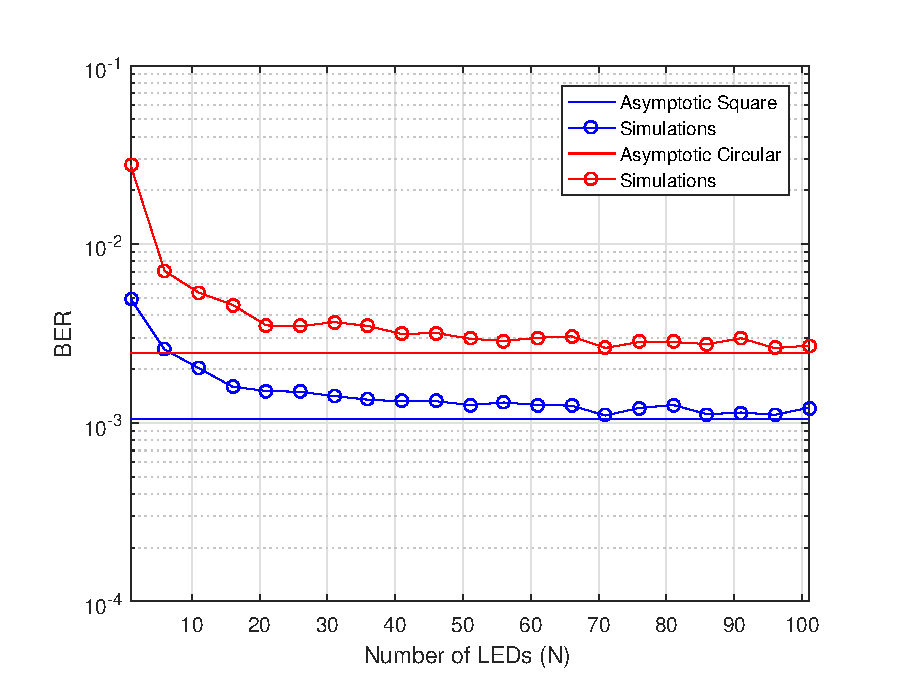
\includegraphics[width=\columnwidth]{berVSNdiffGeom}
     %   \caption{Square BPP}
\label{fig1:subfig2}
    \end{subfigure}
\end{figure}
\vfill
 \textcolor{blue}{ BER can be used to estimate the cost of the system in terms of the number of LEDs}
\end{frame}

\subsection{Optimal Power Allocation for Uniform Illumination}
\begin{frame}
\centering
\vfill
Optimal Power Allocation for Uniform Illumination in VLC Systems
\vfill
\end{frame}
\begin{frame}
\frametitle{\,}
\framesubtitle{Optimal Power Allocation for Uniform Illumination in VLC Systems}
\begin{list}{}{}
\vfill
\item<1-> Given a distribution of source LEDs, How to find the optimum power allocation for uniform illuminance ?  \\ 
\vfill
\vspace{.2in}
\item<2-> Minimize the variance of the received power
\begin{equation}
\begin{aligned}
& \underset{P_{t_i}}{\text{minimize}}
& & \mathbb{E}\sbrak{\brak{P_{r_j}-\mathbb{E}\sbrak{P_{r_j}}}^2} \nonumber
\end{aligned}
\end{equation}
\vfill
\item<3-> 
\footnotesize{
\begin{align}
var(P_{r_j})&=\frac{1}{2}\sum_{i=1}^N \brak{\frac{2\sum_{j=1}^KH_{ij}^2}{K}-\frac{2\brak{\sum_{j=1}^KH_{ij}}^2}{K^2}} P_{t_i}^2 \nonumber \\
            &\qquad + 2 \sum_{u=1}^N \sum_{v=i+1}^{N} \lbrak{\frac{2\sum_{j=1}^KH_{uj}H_{vj}}{K} } \nonumber \\
             &\qquad\qquad \rbrak{-\frac{2\brak{\sum_{j=1}^KH_{uj}}\brak{\sum_{j=1}^KH_{vj}}}{K^2}} P_{t_u}P_{t_v} \nonumber
\end{align}
}
\vfill
\end{list} 
\end{frame}

\begin{frame}
\frametitle{\,}
\framesubtitle{Optimal Power Allocation for Uniform Illumination in VLC Systems}
\begin{list}{}{}
\vfill
\item<1-> The objective function is expressed in quadratic form as
\begin{equation}
\label{var_obj}
\begin{aligned}
& \underset{x}{\text{minimize}}
& & \frac{1}{2}\textbf{x}^T\mathcal{P}\textbf{x}\\
& \text{subject to}
& & \mathcal{G}\textbf{x} \succeq \textbf{0}\\
& & &\mathcal{A}\textbf{x}=P
\end{aligned}\nonumber
\end{equation}
where $\mathcal{G}=diag\brak{-1,\cdots,-1}$, $\mathcal{A}=\sbrak{1,\cdots,1}$ and elements $\beta_{ij}$ of matrix $\mathcal{P}$ is given by
\begin{equation}
\beta_{ij}=
\begin{cases}
\frac{2\sum_{p=1}^Ka_{ip}^2}{K}-\frac{2\brak{\sum_{p=1}^Ka_{ip}}^2}{K^2}, & i=j\\
\frac{2\sum_{p=1}^Ka_{ip}a_{jp}}{K}-\frac{2\brak{\sum_{p=1}^Ka_ip}\brak{\sum_{p=1}^Ka_jp}}{K^2}, & i \neq j\\
\end{cases}\nonumber
\end{equation}
\vfill
\item<2>
\textcolor{blue}{ Numerically solved using quadratic programming (QP)
through the solvers.qp command in Python using CVXOPT solver.}
\vfill
\end{list} 
\end{frame}

\begin{frame}
\frametitle{\,}
\framesubtitle{Optimal Power Allocation for Uniform Illumination in VLC Systems}

\begin{figure}
\centering
\begin{subfigure}{0.33\columnwidth}
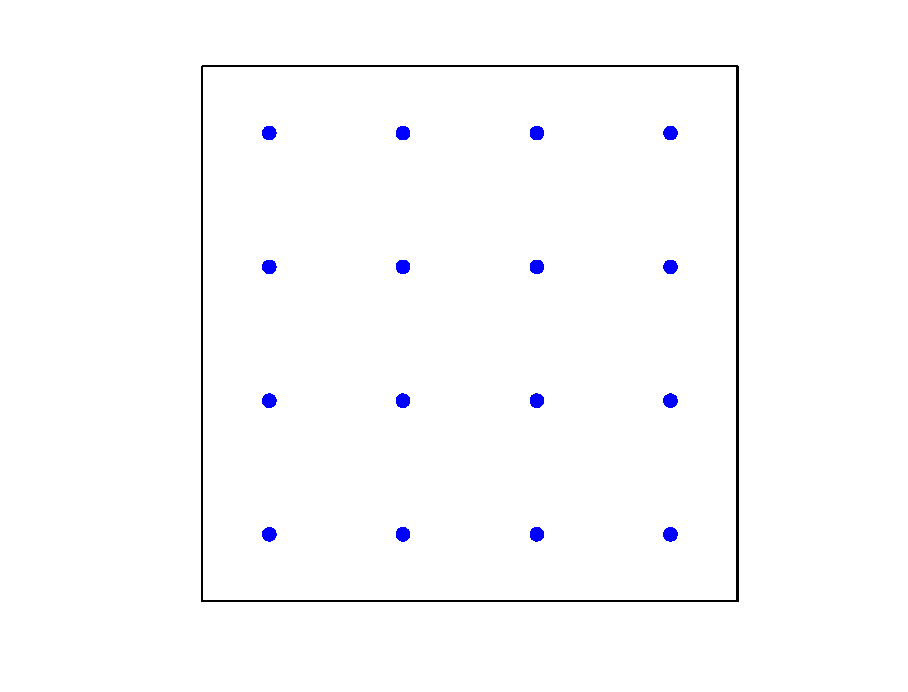
\includegraphics[width=\columnwidth]{c4_deploy_sq}
\caption{Square Array }
\end{subfigure}~
\begin{subfigure}{0.33\columnwidth}
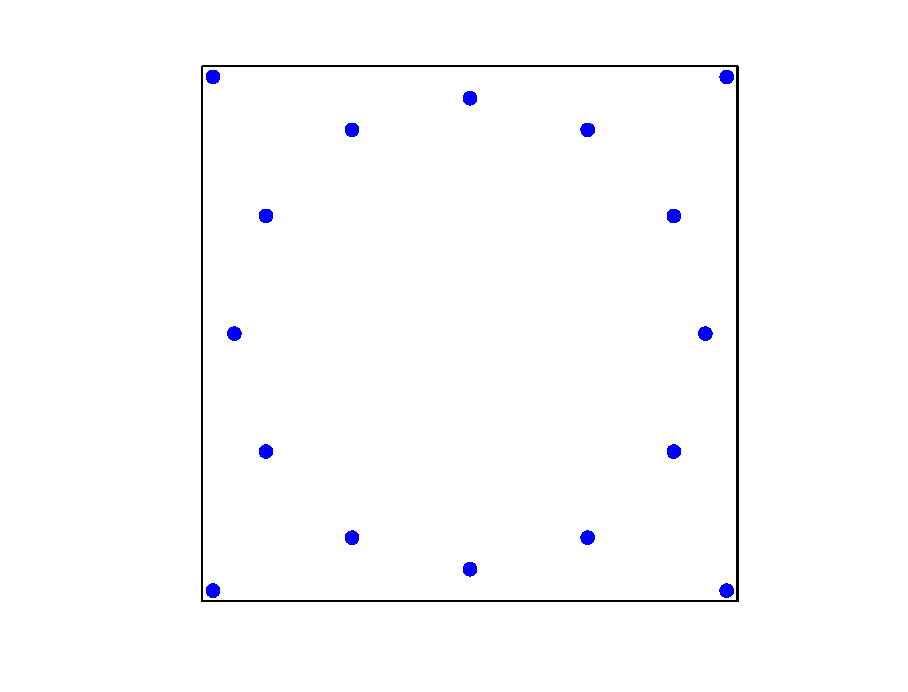
\includegraphics[width=\columnwidth]{c4_deploy_cirsq}
\caption{Circle Square }
\end{subfigure}~
\begin{subfigure}{0.33\columnwidth}
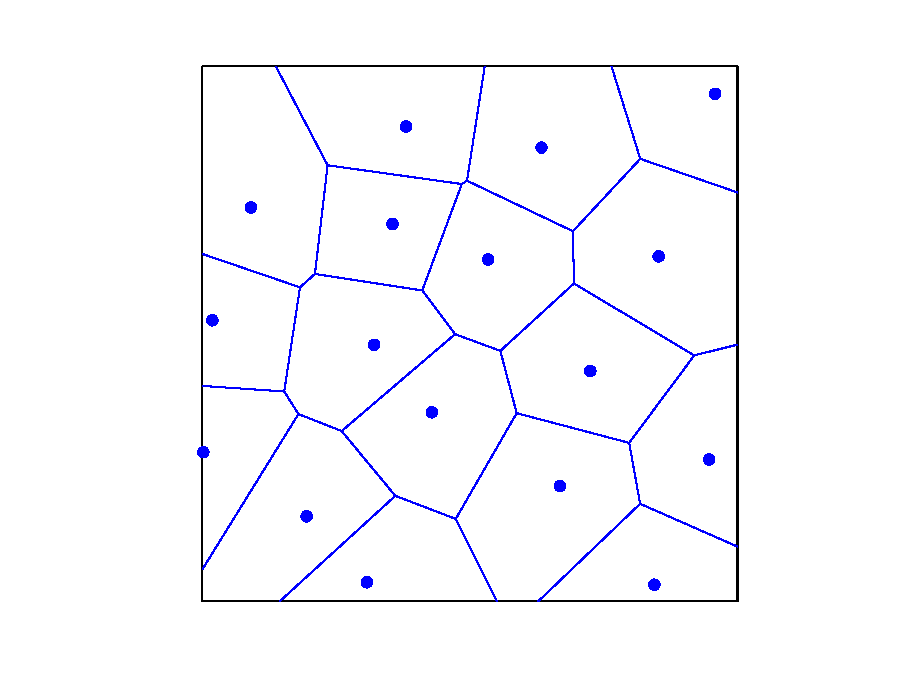
\includegraphics[width=\columnwidth]{c4_deploy_hcpp}
\caption{Realization of HCPP}
\end{subfigure}
\end{figure}
\end{frame}

\begin{frame}
\frametitle{\,}
\framesubtitle{Optimal Power Allocation for Uniform Illumination in VLC Systems}
\begin{figure}[!]
\centering
\begin{subfigure}{0.3\columnwidth}
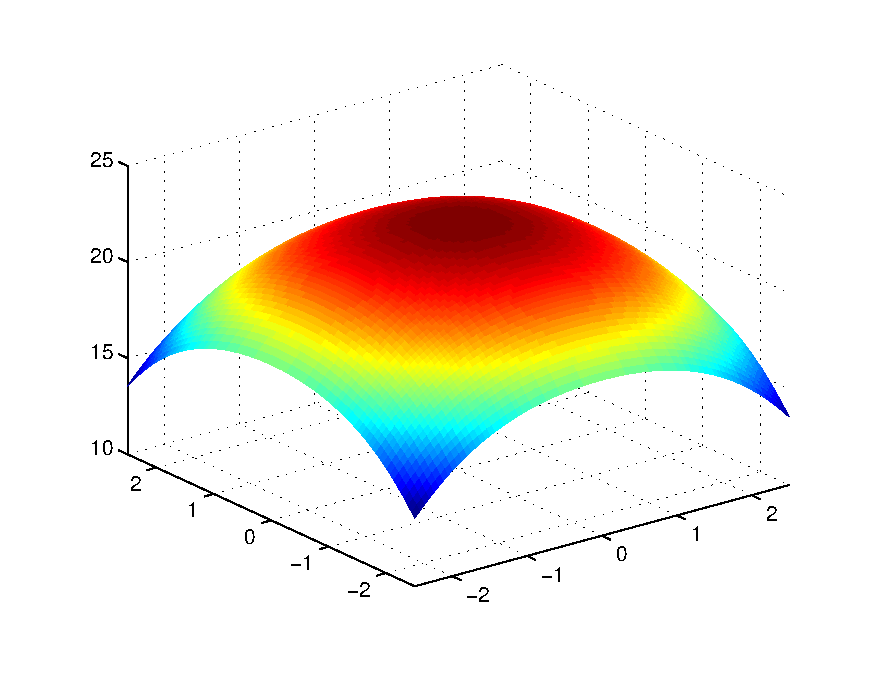
\includegraphics[width=\columnwidth]{c4_sqArr_SNR_Eq}
\caption{Square array with equal power}
\end{subfigure}~
\begin{subfigure}{0.3\columnwidth}
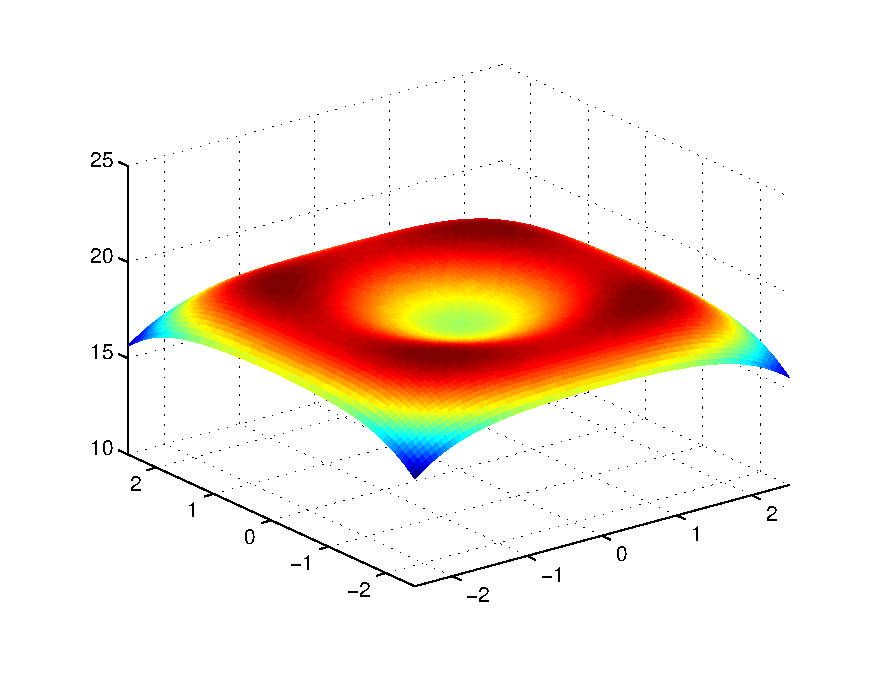
\includegraphics[width=\columnwidth]{c4_cirSq_SNR_Eq}
\caption{Circle square with equal power}
\end{subfigure}~
\begin{subfigure}{0.3\columnwidth}
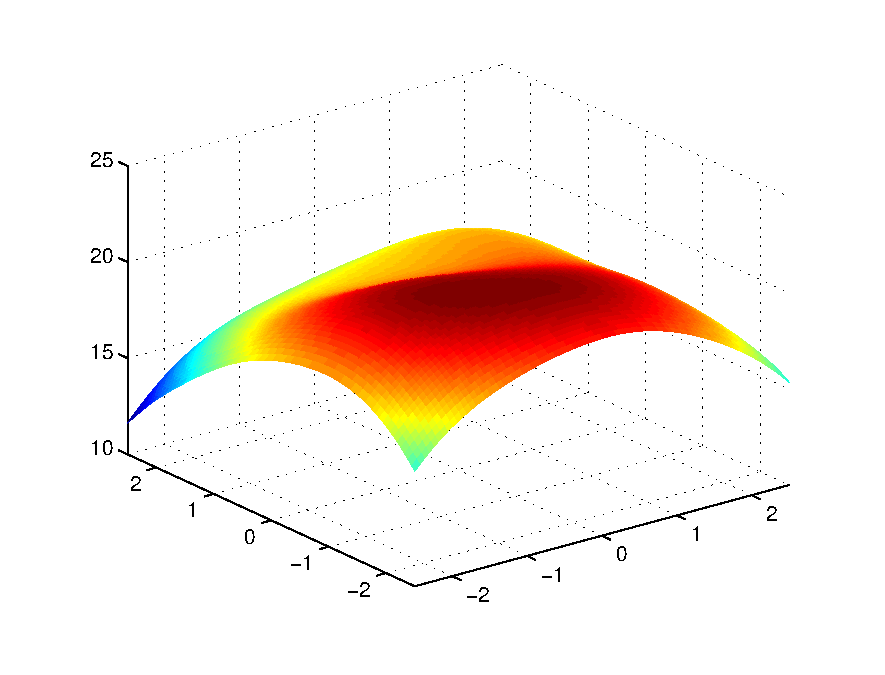
\includegraphics[width=\columnwidth]{c4_hcpp_SNR_Eq}
\caption{HCPP with equal power}
\end{subfigure}
\\
\begin{subfigure}{0.3\columnwidth}
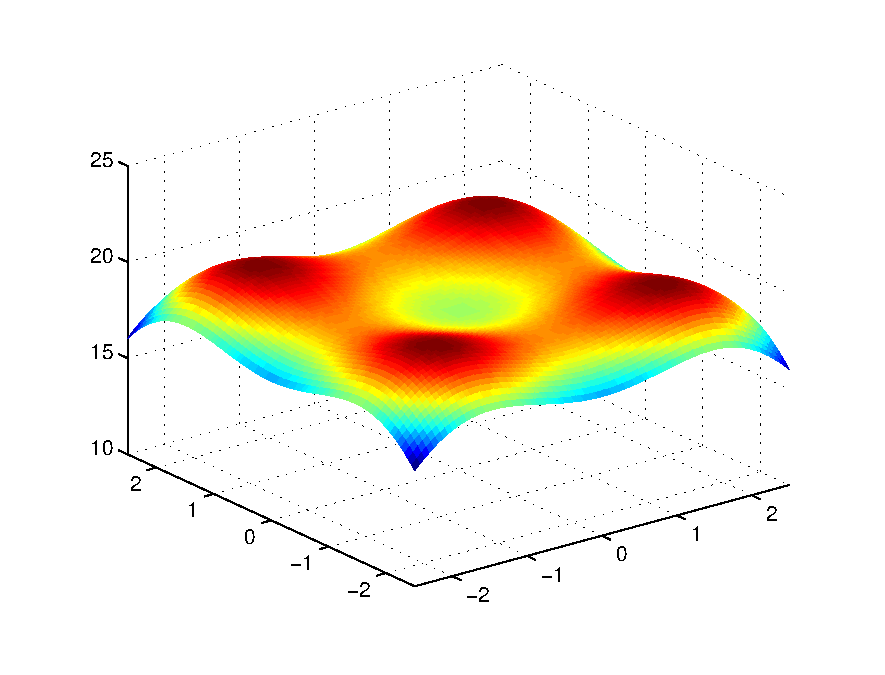
\includegraphics[width=\columnwidth]{c4_sqArr_SNR_opt}
\caption{Square array with optimum power}
\end{subfigure}~
\begin{subfigure}{0.3\columnwidth}
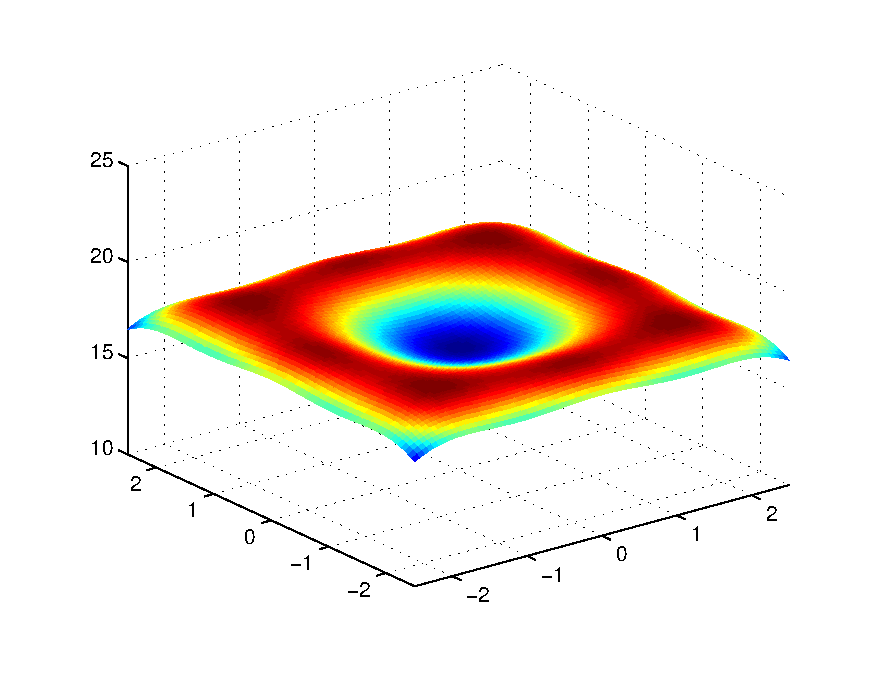
\includegraphics[width=\columnwidth]{c4_cirSq_SNR_opt}
\caption{Circle square with optimum power}
\end{subfigure}~
\begin{subfigure}{0.3\columnwidth}
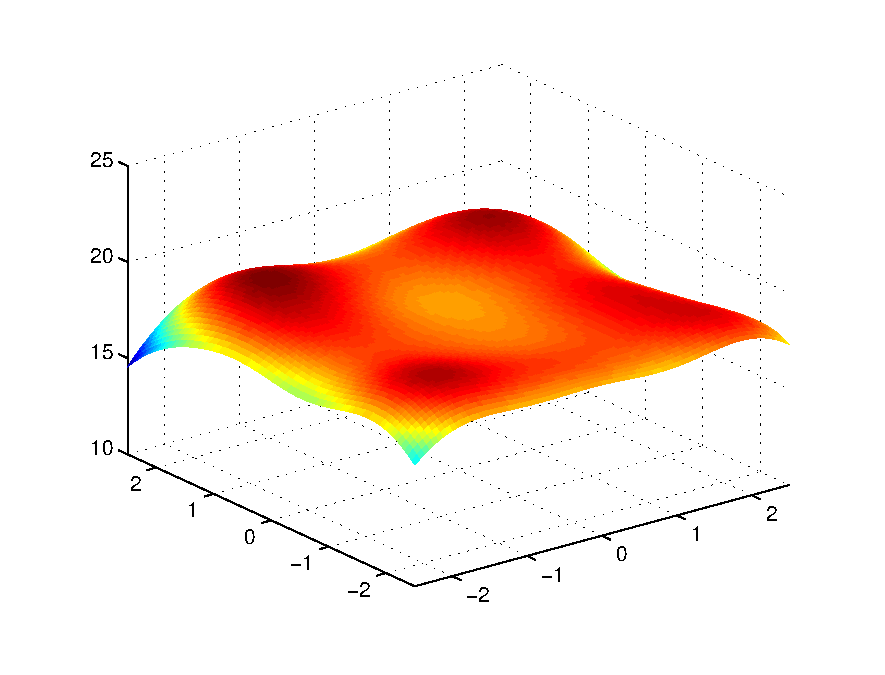
\includegraphics[width=\columnwidth]{c4_hcpp_SNR_opt}
\caption{HCPP with optimum power}
\end{subfigure}
%       \caption{SNR profiles for different geometries. }
    
\label{fig:SNR_profiles}
\end{figure}
\end{frame}


\begin{frame}
\frametitle{\,}
\framesubtitle{Optimal Power Allocation for Uniform Illumination in VLC Systems}
\vfill
\begin{table}[]
\centering
\caption{Variance of received power}
\begin{tabular}{|c|c|c|c|}
 \hline
 & Equal power & Heuristic power & Optimum power   \\
 \hline  
Square Array & 6.4414e-15 & 6.5287e-16 & 6.3785e-16   \\
 \hline 
Circle Square & 3.0134e-15 & 1.1267e-15 &  8.0382e-16  \\
 \hline
BPP & 5.1986e-14 & 3.9660e-14 &  9.8679e-15 \\
 \hline
HCPP  & 2.2504e-14  & 1.2721e-14 &  2.2736e-15 \\
 \hline
\end{tabular}
\end{table}
\vfill
\begin{table}[]
\centering
\caption{Quality factor}
\begin{tabular}{|c|c|c|c|}
 \hline
 & Equal power & Heuristic power & Optimum power   \\
 \hline  
Square Array & 1.34 & 3.30 & 3.28   \\
 \hline 
Circle Square & 3.79 & 4.48 &  5.06 \\
 \hline
BPP & 1.27 & 2.80 &  3.49 \\
 \hline
HCPP  & 1.49  & 3.27 &  4.73 \\
 \hline
\end{tabular}
\end{table}
\vfill
\end{frame}

\begin{frame}
\vfill
\begin{figure}
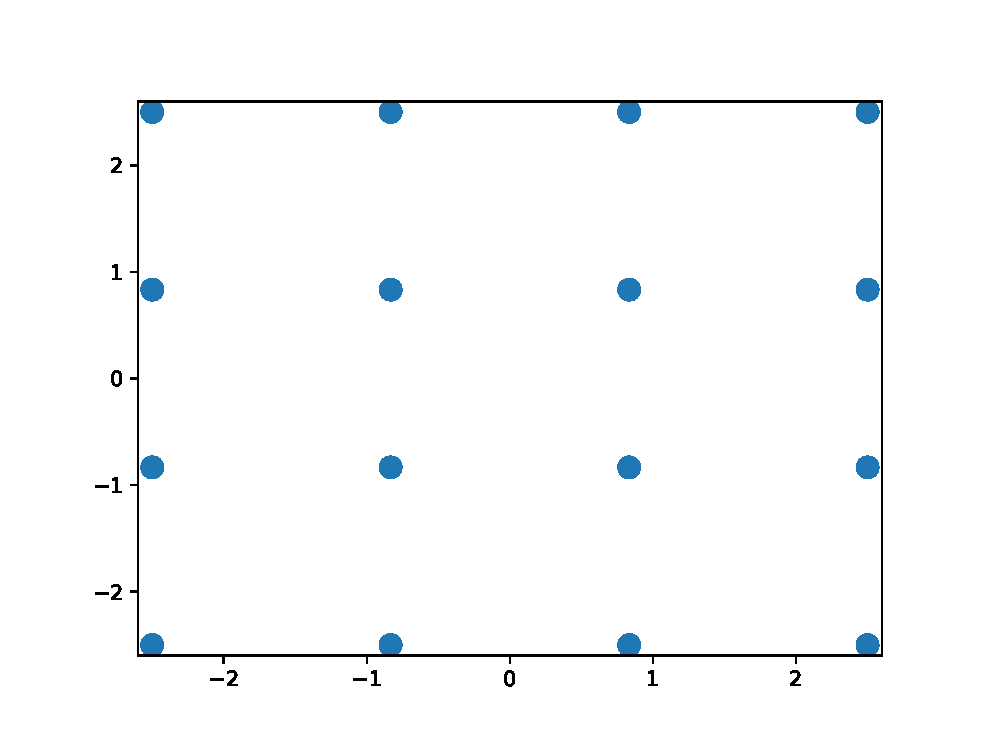
\includegraphics[scale=.25]{sq_opt_loc}
\end{figure}
\vfill
\begin{table}[]
\centering
\caption{Quality factor}
\begin{tabular}{|c|c|c|c|}
 \hline
 & Equal power & Heuristic power & Optimum power   \\
 \hline  
Square Array & 1.34 & 3.30 & 3.28   \\
 \hline 
Circle Square & 3.79 & 4.48 &  5.06 \\
 \hline
BPP & 1.27 & 2.80 &  3.49 \\
 \hline
HCPP  & 1.49  & 3.27 &  4.73 \\
 \hline
\textcolor{blue}{$\underset{optimum location}{\text{Square Array}}$} & \textcolor{blue}{2.62}  & \textcolor{blue}{10.78} &  \textcolor{blue}{11.55} \\
 \hline
\end{tabular}
\end{table}
\vfill
\end{frame}

\begin{frame}
\begin{figure}[!]
\centering
\begin{subfigure}{0.5\columnwidth}
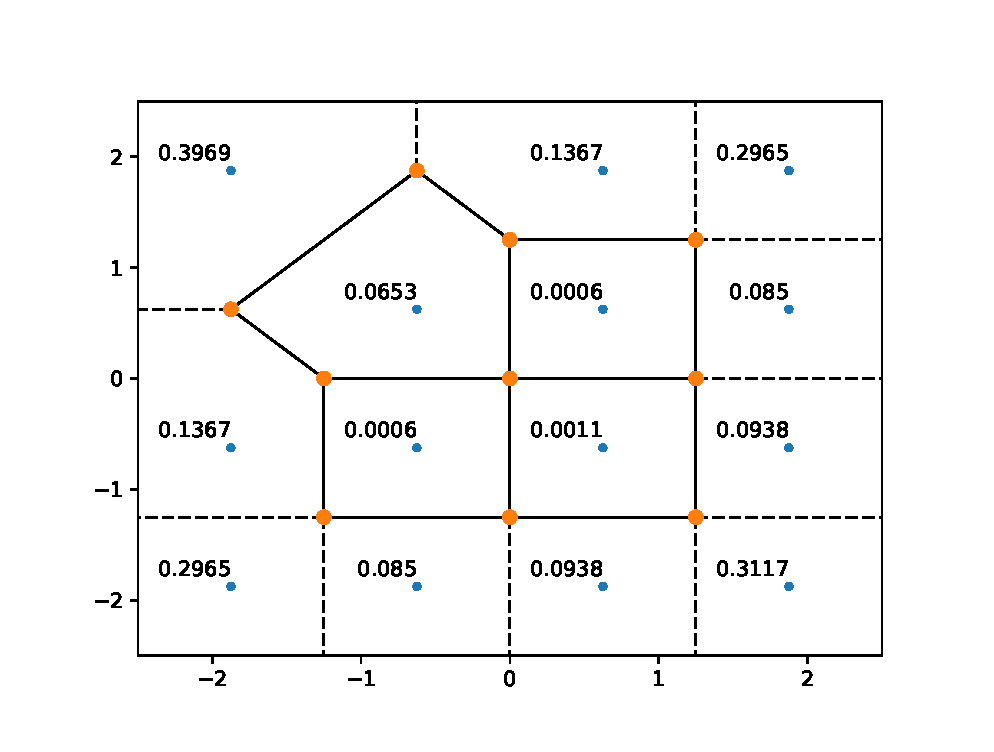
\includegraphics[width=\columnwidth]{sqarr_pwr}
\caption{Square array with optimum power allocation}
\end{subfigure}~
\begin{subfigure}{0.485\columnwidth}
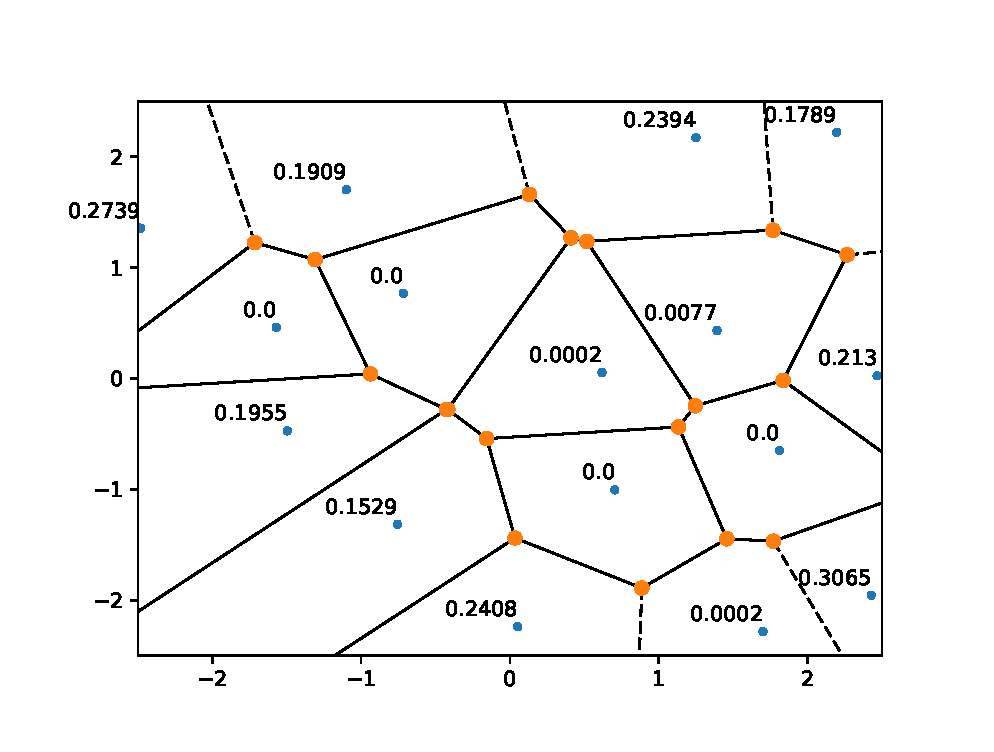
\includegraphics[width=\columnwidth]{hcpp_pwr}
\caption{HCPP realization with optimum power allocation}
\end{subfigure}
\label{fig:SNR_profiles}
\end{figure}
\end{frame}

\begin{frame}
\frametitle{Publications}
\begin{enumerate}
\item
G. V. S. S. Praneeth Varma, Rayapati Sushma, Vandana Sharma, Abhinav Kumar, and G. V. V. Sharma, ``Power allocation for uniform illumination with stochastic LED arrays,'' Optics Express 
 \textbf{25}(8), 8659--8669 (2017).

\item
G. V. S. S. Praneeth Varma, Abhinav Kumar, and G. V. V. Sharma, ``Resource Allocation for Visible Light
Communication using Stochastic Geometry,'' (Submitted).

\item
G. V. S. S. Praneeth Varma, Abhinav Kumar, and G. V. V. Sharma, ``Resource Allocation for Visible Light
Communication using Stochastic Geometry,'' (Submitted).


%\item
%G. V. S. S. Praneeth Varma, ``Optimum Power Allocation for Uniform
%Illuminance in Visible Light Communication Systems,'' (In preparation).

\end{enumerate}
\end{frame}
%\begin{frame}
%\frametitle{More problems}
%\begin{itemize}
%\item<1-> Given a random distribution of source LEDs, what is the optimum power allocation for uniform illuminance ? \\
%\textbf{Can be solved framing it as optimization problem.} (In progress)
%\vfill
%\item<2-> If the SNR distribution is not uniform, can BER analysis be done as above at any location of photo-detector ? \\
%\textbf{Yes. Need to find the distribution of $r_{ij}$}. (In progress)
%\vfill
%\item<3-> The dominant factor in the VLC system is shot noise, which is dependent on the received power at the photo-detector. Hence the effect of noise on the performance of VLC is significant. 
%\vfill
%\item<4-> Inter-symbol interference (ISI) in VLC system is significant. Can the equalization techniques in conventional wireless system be directly applied to VLC ? If not, how do you address it ?
%\end{itemize} 
%\end{frame}

\section{References}
\begin{frame}
\frametitle{References}
\begin{itemize}
 \vfill
\item
J.~Kahn and J.~Barry, ``Wireless infrared communications,'' Proc. IEEE  \textbf{85}(2), 265--298 (1997).
 \vfill
\item
T.~Komine and M.~Nakagawa, ``Fundamental analysis for visible-light
  communication system using led lights,'' IEEE Trans. Consum. Electron.  \textbf{50}(1), 100--107 (2004).
  \vfill
\item
Z.~Wang, C.~Yu, W.-D. Zhong, J.~Chen, and W.~Chen, ``Performance of a novel led
  lamp arrangement to reduce snr fluctuation for multi-user visible light
  communication systems,'' Opt. Express \textbf{20}(4), 4564--4573 (2012).
 \vfill
\item
S.~Srinivasa and M.~Haenggi, ``Distance {D}istributions in {F}inite {U}niformly
  {R}andom {N}etworks: {T}heory and {A}pplications,'' IEEE Trans. Veh. Technol. \textbf{59}(2), 940--949 (2010).
  \vfill
\item
J.~Ding, Z.~Huang, and Y.~Ji, ``Evolutionary algorithm based power coverage
  optimization for visible light communications,'' IEEE Commun. Lett. \textbf{16}(4), 439--441 (2012).
 \vfill
\end{itemize}
\end{frame}

\begin{frame}
\frametitle{References}
\begin{itemize}
 \vfill
\item
Y.~Liu, Y.~Peng, Y.~Liu, and K.~Long;, ``Optimization of receiving power
  distribution using genetic algorithm for visible light communication,''
  Proc. SPIE 9679, Optical Fiber Sensors and Applications \textbf{9679},96790I (2015).
 \vfill
\item
H.~Zheng, J.~Chen, C.~Yu, and M.~Gurusamy, ``Inverse design of led arrangement
  for visible light communication systems,'' Opt. Commun. \textbf{382}, 615--623, (2017).
  \vfill
\item
Sourav Pal, ``Optimization of LED array for uniform illumination over a target plane by evolutionary programming,'' Appl. Opt. \textbf{54}(27), 8221--8227 (2015). 
 \vfill
\item
  P. Lei, Q. Wang, and H. Zou,``Designing LED array for uniform illumination based on local search algorithm,'' J. Europ. Opt. Soc. Rap. Public. \textbf{9}, 14014 (2014).
   \vfill
\item
Y.~Chen, C.~W. Sung, S.-W. Ho, and W.~S. Wong, ``Ber analysis for interfering
  visible light communication systems,'' in International Symposium on
  Communication Systems , Networks and Digital Signal Processing 564--570 (2016).
 \vfill
%\end{thebibliography}
\end{itemize}

\end{frame}

\begin{frame}
\centering
\textcolor{blue}{ \LARGE {Thank You}}
\end{frame}

\begin{frame}
\frametitle{\,}
\framesubtitle{Proof for asymptotic BER}
\begin{equation}
\label{ber_cond_one}
P_e  = \mathbb{E}_{\Phi}\sbrak{\textit{Q}\brak{\frac{RC_1\sum_{i=1}^N V_i}{ \sigma_0}}}
\end{equation}
%
{\textit{Jensens Inequality:}}
If $X$ is a random variable (RV) and $f$ is a convex function, then , 
\begin{equation}
f\brak{\mathbb{E}\sbrak{X}} \leq \mathbb{E}\sbrak{f\brak{X}}
\label{jensen}
\end{equation}
%
%
\begin{equation}
\label{pe_jensen}
P_e  \geq \textit{Q}\brak{ \mathbb{E}_{\Phi}\sbrak{\frac{RC_1\sum_{i=1}^NV_i}{\sigma_0}}}
\end{equation}
%
since $Q\brak{\cdot}$ is convex.
%\end{lemma}
%
\end{frame}
\begin{frame}

\begin{lemma}
Consider random variables X and Y where Y either has no mass at 0 (discrete) or has support
$[0,\infty )$. Then 
\begin{equation}
\mathbb{E}\sbrak{f\brak{X,Y}} \approx f\brak{\mathbb{E}\sbrak{X},\mathbb{E}\sbrak{Y}} 
\end{equation}
\end{lemma}
%Approximations for $\mathbb{E}\sbrak{\frac{X}{Y}}$ using first order Taylor
%expansions is given by 
\begin{corollary}
\begin{align}
\label{exp_ratio}
\mathbb{E}\sbrak{\frac{X}{Y}} &\approx \frac{\mathbb{E}\sbrak{X}}{\mathbb{E}\sbrak{Y}}
\\
\mathbb{E}\sbrak{X^2} &\approx  \brak{\mathbb{E}\sbrak{X}}^2
\label{schwartz}
\end{align}
\end{corollary}

\end{frame}
\begin{frame}
%
Since $\sigma_0 > 0$, using \eqref{exp_ratio} and \eqref{schwartz} in \eqref{pe_jensen},
%
\begin{align}
\textit{Q}\brak{ \mathbb{E}_{\Phi}\sbrak{\frac{RC_1\sum_{i=1}^NV_i}{\sigma_0}}} &\approx \textit{Q}\brak{\frac{RC_1\sum_{i=1}^N \mathbb{E}_{\Phi}\sbrak {V_i}}{ \mathbb{E}_{\Phi}\sbrak{\sigma_0}}}
\nonumber \\
&= \textit{Q}\brak{\frac{RC_1\sum_{i=1}^N \mathbb{E}_{\Phi}\sbrak {V_i}}{ \sqrt{\mathbb{E}_{\Phi}\sbrak{\sigma_0^2}}}}
\end{align}
resulting in
\begin{equation}
P_e \gtrapprox \textit{Q}\brak{\frac{RC_1\sum_{i=1}^N \mathbb{E}_{\Phi}\sbrak {V_i}}{ \sqrt{\mathbb{E}_{\Phi}\sbrak{\sigma_0^2}}}}
\end{equation}
%
%
\end{frame}

\begin{frame}
\frametitle{\,}
\framesubtitle{BER Analysis for Square BPP}
  \begin{align}
   \mathbb{E}_{\Phi}\sbrak{r_i^{\alpha}} & =\int_{-\infty}^{\infty}r^{\alpha}f_{r_i}(r)dr \nonumber \\
   & = \int_{0}^{R_i}r^{\alpha}\frac{2\pi r}{W}\frac{\brak{1-p}^{N-i}p^{i-1}}{\mathcal{B}\brak{N-i+1,
   i}}dr \nonumber \\
   &\quad  +\int_{R_i}^{R_c}r^{\alpha}\frac{2\brak{\pi-4\theta} r}{W}\frac{\brak{1-q}^{N-i}q^{i-1}}{\mathcal{B}\brak{N-i+1,i}}dr \nonumber
   \\
    & =   \mathcal{I}_1 + \mathcal{I}_2 \nonumber
   \end{align}
   %
   \end{frame}
   \begin{frame}
   where
   \begin{align}
    \mathcal{I}_1& = \int_{0}^{R_i}r^{\alpha}\frac{2\pi r}{W}\frac{\brak{1-p}^{N-i}p^{i-1}}{\mathcal{B}\brak{N-i+1,i}}dr \nonumber \\
%   & = \int_{0}^{R_i}r^{\alpha}\frac{2\pi r}{W\mathcal{B}\brak{N-i+1,i}}\sum_{k=0}^{N-i}\binom{N-i}{k}(-1)^kp^{k+i-1}dr\\
   & = \frac{2\pi }{W\mathcal{B}\brak{N-i+1,i}}\sum_{k=0}^{N-i}\binom{N-i}{k}(-1)^k\brak{\frac{\pi}{W}}^{k+i-1}
  \nonumber \\
  &\quad \times\int_{0}^{R_i}r^{2\brak{k+i+\alpha/2+1/2}} dr \nonumber
   %\end{align}
   %Following a change of variables,
   %\begin{align}
      %\mathcal{I}_1 & = \frac{\pi }{W\mathcal{B}\brak{N-i+1,i}}\sum_{k=0}^{N-i}\binom{N-i}{k}(-1)^k\brak{\frac{\pi}{W}}^{k+i-1}
     %\nonumber \\
     %& \quad \int_{0}^{R_i^2}t^{\brak{k+i+\alpha/2-1}} dt 
     \\
       & = \frac{1 }{\mathcal{B}\brak{N-i+1,i}}\sum_{k=0}^{N-i}\frac{\binom{N-i}{k}(-1)^k}{k+i+\alpha/2}\brak{\frac{\pi}{W}}^{k+i}R_i^{2\brak{k+i}+\alpha}
       \\
   %\end{align}
%Also,
%    \begin{align}
    \mathcal{I}_2 & = \int_{R_i}^{R_c}r^{\alpha}\frac{2\brak{\pi-4\theta} r}{W}\frac{\brak{1-q}^{N-i}q^{i-1}}{\mathcal{B}\brak{N-i+1,i}}dr \nonumber \\
   %& = \int_{R_i}^{R_c}r^{\alpha}\frac{2\brak{\pi-4\theta} r}{W\mathcal{B}\brak{N-i+1,i}}\sum_{k=0}^{N-i}\binom{N-i}{k}(-1)^kq^{k+i-1}dr\\
   & = \frac{1}{\mathcal{B}\brak{N-i+1,i}}\sum_{k=0}^{N-i}\frac{\binom{N-i}{k}(-1)^k}{W^{k+i}}
   R_i^{2\brak{k+i}+\alpha-1} \nonumber \\
   &\quad \times \int_{0}^{\frac{\pi}{4}} \frac{2\brak{\pi-4\theta}\brak{\pi-4\theta+2\sin\brak{2\theta}}^{k+i-1} }{\cos^{2\brak{k+i}+\alpha-1}\brak{\theta}}\,d \theta
   \end{align}
   upon substituting $R_i = r \cos \theta$.
%\section{Evaluating $\mathbb{E}_{\Phi}\sbrak{V_i}$}   
\label{app_Pe}
 %   
 \end{frame}
 \begin{frame}
 For simplifying the analysis, using the approximation
\begin{equation}
\sum_{j=1}^N\mathbb{E}_{\Phi}\sbrak{r_j^{\alpha}} \approx \sum_{j=1}^Nr_j^{\alpha}
\end{equation}
in \eqref{variable_Vi},
   \begin{align}
   \mathbb{E}_{\Phi}\sbrak{V_i}&=\frac{1}{\sum_{j=1}^N\mathbb{E}_{\Phi}\sbrak{r_j^{\alpha}} }\mathbb{E}_{\Phi}\sbrak{\frac{r^{\alpha}}{\brak{\sqrt{r^2+h^2}}^{m+3}}} \\
%   & =\int_{-\infty}^{\infty}r^{\alpha}f_{r}(r)dr\\
   %& = \frac{1}{\sum_{j=1}^N\mathbb{E}_{\Phi}\sbrak{r_j^{\alpha}} } \quad \times  \nonumber\\
   %& \quad  \lbrak{\int_{0}^{R_i}\frac{r^{\alpha}}{\brak{\sqrt{r^2+h^2}}^{m+3}}\frac{2\pi r}{W}\frac{\brak{1-p}^{N-i}p^{i-1}}{\mathcal{B}\brak{N-i+1,i}}dr}  \nonumber\\ 
     %&  \rbrak{+\int_{R_i}^{R_c}\frac{r^{\alpha}}{\brak{\sqrt{r^2+h^2}}^{m+3}}\frac{2\brak{\pi-4\theta} r}{W}\frac{\brak{1-q}^{N-i}q^{i-1}}{\mathcal{B}\brak{N-i+1,i}}dr}  \\
    & =  \frac{ \mathcal{J}_1 + \mathcal{J}_2}{\sum_{j=1}^N\mathbb{E}_{\Phi}\sbrak{r_j^{\alpha}} }
   \end{align}
   \end{frame}
   \begin{frame}
  where
   \begin{align}
    \mathcal{J}_1& = \int_{0}^{R_i}\frac{r^{\alpha}}{\brak{\sqrt{r^2+h^2}}^{m+3}}\frac{2\pi r}{W}\frac{\brak{1-p}^{N-i}p^{i-1}}{\mathcal{B}\brak{N-i+1,i}}dr 
%   & = \int_{0}^{R_i}\frac{r^{\alpha}}{\brak{\sqrt{r^2+h^2}}^{m+3}}\frac{2\pi r}{W\mathcal{B}\brak{N-i+1,i}}
   \nonumber \\
   %& \quad \times \sum_{k=0}^{N-i}\binom{N-i}{k}(-1)^kp^{k+i-1}dr\\
   %& = \frac{1 }{\mathcal{B}\brak{N-i+1,i}}\sum_{k=0}^{N-i}\binom{N-i}{k}(-1)^k\brak{\frac{\pi}{W}}^{k+i}
   %\nonumber \\
   %& \quad \times \int_{0}^{R_i}2r\frac{r^{2\brak{k+i+\alpha/2-1}}}{\brak{\sqrt{r^2+h^2}}^{m+3}}dr\\ 
      %& = \frac{1}{\mathcal{B}\brak{N-i+1,i}}\sum_{k=0}^{N-i}\binom{N-i}{k}(-1)^k\brak{\frac{\pi}{W}}^{k+i}\frac{h^{2\brak{k+i+\alpha/2-1}}}{h^{m+1}}
      %\nonumber 
      %\\
      %& \quad \times \int_{0}^{R_i^2/h^2}\frac{t^{\brak{k+i+\alpha/2-1}}}{\brak{\sqrt{1+t}}^{m+3}}dt \\
       & = \frac{R_i^{\alpha}}{h^{m+3}\mathcal{B}\brak{N-i+1,i}}\sum_{k=0}^{N-i}\binom{N-i}{k}(-1)^k\brak{\frac{\pi R_i^2}{W}}^{k+i}
       \nonumber \\
       & \quad \times \int_{0}^{R_i^2/h^2}\frac{t^{\brak{k+i+\alpha/2}-1}}{\brak{1+t}^\frac{m+3}{2}}dt
       \label{J_1_app}
   \end{align}
   %
after some algebra.   
\end{frame}
\begin{frame}
\footnotesize{
   \begin{align}
\int_{0}^{u}\frac{x^{\mu-1}}{\brak{1+\beta x}^{\nu}}dx=\frac{u^{\mu}}{\mu}  \,_2F_1\brak{\nu,\mu;1+\mu;-\beta u}
\qquad \sbrak{\abs{arg\brak{1+\beta u}} < \pi, Re\mu>0}
\end{align}
}
%
Substituting the above in \eqref{J_1_app},
 \begin{align}
    \mathcal{J}_1& = \frac{h^{\alpha}}{h^{m+3}\mathcal{B}\brak{N-i+1,i}}\sum_{k=0}^{N-i}\binom{N-i}{k}(-1)^k\brak{\frac{\pi h^2}{W}}^{k+i}
   \nonumber \\
   &\quad \times \,_2F_1\brak{\frac{m+3}{2},\brak{k+i+\alpha/2},k+i+\alpha/2+1;-\frac{R_i^2}{h^2}} 
   \end{align}
   Similarly, 
    \begin{align}
   \mathcal{J}_2 & = \int_{R_i}^{R_c}\frac{r^{\alpha}}{\brak{\sqrt{r^2+h^2}}^{m+3}}\frac{2\brak{\pi-4\theta} r}{W}\frac{\brak{1-q}^{N-i}q^{i-1}}{\mathcal{B}\brak{N-i+1,i}}dr \nonumber \\
   %& = \int_{R_i}^{R_c}\frac{r^{\alpha}}{\brak{\sqrt{r^2+h^2}}^{m+3}}\frac{2\pi r}{W\mathcal{B}\brak{N-i+1,i}}
   %\nonumber \\
   %&\quad \times \sum_{k=0}^{N-i}\binom{N-i}{k}(-1)^kq^{k+i-1}dr\\
   & = \frac{1}{\mathcal{B}\brak{N-i+1,i}}\sum_{k=0}^{N-i}\frac{\binom{N-i}{k}(-1)^k}{W^{k+i}}
  \nonumber \\
  & \quad \times   \int_{0}^{\frac{\pi}{4}} \frac{2\brak{\pi-4\theta}R_i^{2\brak{k+i}+\alpha-1}}{\cos^{2\brak{k+i-2}+\alpha-m}\brak{\theta}}
   \frac{\brak{\pi -4\theta+2\sin\brak{2\theta}}^{k+i-1}}{\brak{\sqrt{R_i^2+h^2\cos^2\brak{\theta}}}^{m+3}} d\theta
      \end{align}
\end{frame}
\begin{frame}
\frametitle{\,}
\framesubtitle{
BER analysis for circular BPP
}   
The probability density function (PDF) of the distance of $i^{th}$ nearest LED location from origin for circular BPP for $0 \leq r \leq R_c$ is given by 
\begin{align}
f_{r_i}	&=
%\frac{2\Gamma\brak{i+1/2}\Gamma\brak{N+1}}{R\Gamma\brak{n}\Gamma\brak{N+3/2}}\frac{\Gamma\brak{N+3/2}\brak{r/R}^{2n-1}\brak{1-(r/R)^2}^{N-n}}{\Gamma\brak{n+1/2}\Gamma\brak{N-n+1}}\\
\frac{2r}{R_c^2 B\brak{i,N-i+1}}\brak{\frac{r^2}{R_c^2}}^{i-1}\brak{1-\frac{r^2}{R_c^2}}^{N-i}
\nonumber \\
%&=\frac{2}{R\mathcal{B}\brak{N-i+1,i}}\brak{r/R}^{2i-1}\sum_{k=0}^{N-i}\binom{N-i}{k}(-1)^{k}(r/R)^{2(k)}\\
%$&=\frac{2r}{R_c^2\mathcal{B}\brak{N-i+1,i}}\sum_{k=0}^{N-i}\binom{N-i}{k}(-1)^{k}(r/R_c)^{2(i+k-1)}
%\end{equation}
%
%Hence,
%
% \begin{align}
 \Rightarrow  \mathbb{E}_{\Phi}\sbrak{r_i^{\alpha}} & =\int_{0}^{\infty}r^{\alpha}f_{r_i}(r)dr \nonumber \\
   & =\int_{0}^{R_c}\frac{2r r^{\alpha}}{R_c^2 B\brak{N-i+1},i} \brak{\frac{r^2}{R_c^2}}^{i-1}
   \brak{1-\frac{r^2}{R_c^2}}^{N-i} dr \nonumber \\
   %& =\int_{0}^{R_c}\frac{2r}{\mathcal{B}\brak{N-i+1,i}}\sum_{k=0}^{N-i}\binom{N-i}{k}(-1)^{k}\frac{r^{2(i+k+\alpha/2-1)}}{R_c^{2(i+k)}} dr\\
    & =\frac{1}{B\brak{N-i+1,i}}\sum_{k=0}^{N-i}\binom{N-i}{k}(-1)^{k}
    \int_{0}^{R_c^2}\frac{t^{i+k+\alpha/2-1}}{R_c^{2(i+k)}} dt \nonumber \\
     & =\frac{R_c^{\alpha}}{B\brak{N-i+1,i}}\sum_{k=0}^{N-i}\frac{\binom{N-i}{k}\brak{-1}^{k}}{\brak{i+k+\frac{\alpha}{2}}} 
   \end{align}
   through a change of variables 
   \end{frame}
   \begin{frame}
   \footnotesize{
\begin{align}
   \mathbb{E}_{\Phi}\sbrak{V_i}&=\frac{1}{\sum_{j=1}^N\mathbb{E}_{\Phi}\sbrak{r_j^{\alpha}} }\mathbb{E}_{\Phi}\sbrak{\frac{r^{\alpha}}{\brak{\sqrt{r^2+h^2}}^{m+3}}} \nonumber \\
   &=\frac{1}{\sum_{j=1}^N\mathbb{E}_{\Phi}\sbrak{r_j^{\alpha}} } \int_{0}^{R_c}\frac{2r}{\mathcal{B}\brak{N-i+1,i}} \sum_{k=0}^{N-i}\binom{N-i}{k}\frac{(-1)^{k}r^{2(i+k+\alpha/2-1)}}{R_c^{2(i+k)}\brak{\sqrt{r^2+h^2}}^{m+3}}dr \nonumber \\
    &=\frac{1}{\mathcal{B}\brak{N-i+1,i}\sum_{j=1}^N\mathbb{E}_{\Phi}\sbrak{r_j^{\alpha}} }  \int_{0}^{R_c^2/h^2} \sum_{k=0}^{N-i}\frac{\binom{N-i}{k}(-1)^{k}h^{2}\brak{h^2t}^{(i+k+\alpha/2-1)}}{R_c^{2(i+k)}h^{m+3}\brak{\sqrt{1+t}}^{m+3}}dt \nonumber \\
    &=\frac{1}{B\brak{N-i+1,i}\sum_{j=1}^N\mathbb{E}_{\Phi}\sbrak{r_j^{\alpha}} } \sum_{k=0}^{N-i}\binom{N-i}{k}\frac{(-1)^{k}h^{2(i+k+\alpha/2)}}{h^{m+3}R_c^{2(i+k)}}
    \nonumber \\
    & \quad \times \int_{0}^{R_c^2/h^2} \!\!\!\!\frac{t^{(i+k+\alpha/2-1)}}{\brak{1+t}^{\brak{m+3}/2}}dt \nonumber \\
     &=\frac{R_c^{\alpha}h^{-(m+3)}}{B\brak{N-i+1,i}\sum_{j=1}^N\mathbb{E}_{\Phi}\sbrak{r_j^{\alpha}}} \nonumber \\
     &\quad \times \sum_{k=0}^{N-i}\frac{\binom{N-i}{k}(-1)^{k}}{\brak{i+k+\frac{\alpha}{2}}}   \, _2F_1\brak{\frac{m+3}{2},i+k+\frac{\alpha}{2};i+k+\frac{\alpha}{2}+1;-\frac{R_c^2}{h^2}}
   \end{align}
}
\end{frame}
\begin{frame}
\frametitle{\,}
\framesubtitle{Formulation of optimization problem}
\begin{equation}
P_{r_j}=\sum_{i=1}^NH_{ij}P_{t_i}
\end{equation}

$var(P_{r_j})=\mathbb{E}\sbrak{\brak{P_{r_j}}^2}-\brak{\mathbb{E}\sbrak{P_{r_j}}}^2$
\footnotesize{
\begin{align}
\brak{\mathbb{E}\sbrak{P_{r_j}}}^2&=\brak{\frac{\sum_{j=1}^KP_{r_j}}{K}}^2\\ \nonumber
&=\brak{\frac{\sum_{j=1}^K\sum_{i=1}^NH_{ij}P_{t_i}}{K}}^2\\ \nonumber
&=\brak{\frac{\sum_{i=1}^N\gamma_iP_{t_i}}{K}}^2 \text{ where } \gamma_i=\sum_{j=1}^KH_{ij}\\ \nonumber
&=\frac{\sum_{i=1}^N\gamma_i^2P_{t_i}^2+2\sum_{i=1}^N\sum_{p=i+1}^{N}\gamma_i\gamma_pP_{t_i}P_{t_p}}{K^2}
\end{align}
}
\end{frame}
\begin{frame}
\footnotesize{
\begin{align}
\mathbb{E}\sbrak{\brak{P_{r_j}}^2}&=\mathbb{E}\sbrak{\brak{\sum_{i=1}^NH_{ij}P_{t_i}}^2}\\ \nonumber
&=\mathbb{E}\sbrak{\sum_{i=1}^N H_{ij}^2P_{t_i}^2 + 2 \sum_{i=1}^N \sum_{q=i+1}^{N} H_{ij}H_{qj}P_{t_i}P_{t_q}}\\ \nonumber
&=\frac{\sum_{j=1}^K\sbrak{\sum_{i=1}^N H_{ij}^2P_{t_i}^2 + 2 \sum_{i=1}^N \sum_{q=i+1}^{N} H_{ij}H_{qj}P_{t_i}P_{t_q}}}{K}\\ \nonumber
&=\frac{\sum_{i=1}^N \mu_{ii} P_{t_i}^2 + 2 \sum_{i=1}^N \sum_{q=i+1}^{N} \mu_{iq} P_{t_i}P_{t_q}}{K}\\
&\qquad \text{ where } \mu_{iq}=\sum_{j=1}^KH_{ij}H_{qj}\\ \nonumber
\end{align}
}
\end{frame}
\begin{frame}
\footnotesize{
\begin{align}
var(P_{r_j})&=\frac{\sum_{i=1}^N \mu_{ii} P_{t_i}^2 + 2 \sum_{i=1}^N \sum_{q=i+1}^{N} \mu_{iq} P_{t_i}P_{t_q}}{K} \nonumber \\
             & \quad- \frac{\sum_{i=1}^N\gamma_i^2P_{t_i}^2+2\sum_{i=1}^N\sum_{p=i+1}^{N}\gamma_i\gamma_pP_{t_i}P_{t_p}}{K^2}  \nonumber \\
            &=\sum_{i=1}^N \frac{\mu_{ii}}{K}-\frac{\gamma_i^2}{K^2} P_{t_i}^2 + 2 \sum_{i=1}^N \sum_{q=i+1}^{N} \frac{\mu_{iq}}{K}-\frac{\gamma_i\gamma_p}{K^2} P_{t_i}P_{t_q} \nonumber \\
            &=\frac{1}{2}\sum_{i=1}^N \brak{\frac{2\sum_{j=1}^KH_{ij}^2}{K}-\frac{2\brak{\sum_{j=1}^KH_{ij}}^2}{K^2}} P_{t_i}^2 \nonumber \\
            &\qquad + 2 \sum_{u=1}^N \sum_{v=i+1}^{N} \lbrak{\frac{2\sum_{j=1}^KH_{uj}H_{vj}}{K} } \rbrak{-\frac{2\brak{\sum_{j=1}^KH_{uj}}\brak{\sum_{j=1}^KH_{vj}}}{K^2}} P_{t_u}P_{t_v} \nonumber \\
            &=\frac{1}{2}\begin{matrix}\begin{bmatrix}P_{t_1},\cdots,P_{t_N}\end{bmatrix}\\\mbox{}\end{matrix}
				\begin{bmatrix} \beta_{11}& \cdots &\beta_{1N} \\
								\vdots &\ddots &\vdots  \\
								\beta_{N1}& \cdots &\beta_{NN}  
								\end{bmatrix} 
				\begin{bmatrix} P_{t_1} \\ \vdots \\ P_{t_N} \end{bmatrix} \nonumber \\
			&=\frac{1}{2}x^T\mathcal{P}x
\end{align}
}
\end{frame}


%\newslide
%{\color{red}
%\begin{multicols}{2}
%\tableofcontents
%\end{multicols}
%}
%\end{slide}
%\section{A list environment}
%\frame{
%\begin{slide}
%\centerslidesfalse
%\frametitle{A list environment}
%
%% The \pause command `splits' the current page at the place it appears, producing two pages, one with everything which
%% came before the \pause command, one containing this and additionally the stuff coming after \pause. When these pages
%% are presented with acrobar reader in full screen mode (or any other viewer with this capability), the presentation
%% will appear to `stop' at the point the \pause command was issued and `resume' in the moment the presenter switches to
%% the next page.
%
%\pause
%
%% As \pause forces a paragraph break, it can not be used to separate a description label from the associated text. For
%% this, we use the (very flexible) \stepwise command. Inside the argument of \stepwise, an arbitrary number of \step
%% commands may occur. \stepwise will produce as many pages as there are \step commands, making the arguments of the
%% \step commands appear ``one by one''.
%
%%\stepwise
%%{%
%%  \begin{description}
%%  \item[foo.] \step{bar.}
%%  \step{\item[baz.]} \step{qux.}
%%  \end{description}
%%  }
%
%
%
%\end{slide}
%}

%\frame{\titlepage}
%\section{Conditionally Gaussian Distributions}
%  %--------------------------------------------------------------------------------
% \frame{
% \frametitle{Teaching}
% 
%% \begin{definition}
%%\label{cond_gauss}
%%\end{definition}
%
%\begin{itemize}
%{\color{red}
%%
% \item Among the top 5 students of the batch (CGPA).
%  \item Has a paper published in COMSNETS 2016 and NCC 2016
%\item A good amount of research work done in the IVth and Vth semester
%\item {\em Got C grade in a couple of courses during this time. Reason: Heavy Course Load.}
%%
%}
%\end{itemize}
%
% 	}
%% 	\section{Problem Definition}
% 	 	 %--------------------------------------------------------------------------------
% 
% \begin{frame}{Student Group: EE 2014 batch}
% 
% 	 	 
%% \frame{
%%  \frametitle{Student Group: EE 2014 batch}
%
%	\begin{itemize}
%	{\color{red}
%%
%\item Started a project in Summer 2015 for Indian Railways electric loco shed.
%\item Automated testing system for traction motor temperature sensor. 
%\item Industry standard work, completed in December 2015
%\item {\em Were unable to work on the project during the semester.  Reason:  Course Load.}
%%\item Piecewise-linear (PL) approximation practically useful 
%%\item Closed form BER expressions for noncoherent PL-DF available
%%\item PL-DF shown (theoretically) to lose half the diversity order 
%  }
%%
%  \end{itemize}
%% 	}
%\end{frame}
%
% 	  %--------------------------------------------------------------------------------
% \frame{
% \frametitle{Student 2: EE 2015}
%
%%\begin{itemize}
%% \item Analyzed the piecewise-linear (PL) combiner for DF cooperation.
%% \end{itemize}
%\begin{itemize}
%{\color{red}
% \item Currently doing a project concieved during the Heritage tour at Golconda fort this semester.
%  \item To estimate the curvature of various archs at Golconda fort through  camera phone images.
%  \item Preliminary results using least squares positive.  {\em No time available during semester to verify results by revisiting Golconda fort}
%}
%\end{itemize}
%
% 	}
% 	  %--------------------------------------------------------------------------------
% 	  \frame{
% 	  	\frametitle{Student 3: EE 2013}
% 	  	
% 	  	%\begin{itemize}
% 	  	% \item Analyzed the piecewise-linear (PL) combiner for DF cooperation.
% 	  	% \end{itemize}
% 	  	\begin{itemize}
% 	  		{\color{red}
% 	  			\item Wins TCS CodeVita contest this month.
% 	  			\item Strong interest in CSE. 
% 	  			\item
% 	  			\em {\em Deserves a double major in CSE department.  No mechanism currently in place to facilitate this.}
% 	  		}
% 	  	\end{itemize}
% 	  	
% 	  }
% 	  
%
% 	  %--------------------------------------------------------------------------------
% 	  \frame{
% 	  	\frametitle{}
% 	  	
% 	  	%\begin{itemize}
% 	  	% \item Analyzed the piecewise-linear (PL) combiner for DF cooperation.
% 	  	% \end{itemize}
%\vspace{2cm}
%\begin{center}
%\color{red}
%\Huge	EE UG Course Credits at Premier Institutes Worldwide 
%\end{center}
%
%
% 	  }
% %--------------------------------------------------------------------------------
%\frame{
%
%\frametitle{UC Berkeley}
%
%\color{red}
%\input{berkeley}
%
%
%\url{http://engineering.berkeley.edu/academics/undergraduate-guide/academic-departments-programs/electrical-engineering-computer-sciences
%	}
%
%%\begin{verbatim}
%%http://engineering.berkeley.edu/academics/undergraduate-guide/academic-departments-programs/electrical-engineering-computer-sciences
%%\end{verbatim}
%
%}
% %--------------------------------------------------------------------------------
%\frame{
%
%\frametitle{Stanford}
%\color{red}
%\input{stanford}
%
%%\begin{vebatim}
%\url{
%	http://web.stanford.edu/group/ughb/cgi-bin/handbook/index.php/Electrical\_Engineering\_Program\#Degree\_Requirements
%	}
%%http://web.stanford.edu/group/ughb/cgi-bin/handbook/index.php/Electrical_Engineering_Program#Degree_Requirements
%%\end{verbatim}
%
%}
% %--------------------------------------------------------------------------------
%\frame{
%
%\frametitle{IIT Bombay}
%\color{red}
%
%\input{iitb}
%
%%\begin{verbatim}
%\url{https://www.ee.iitb.ac.in/web/academics/btech\_courses\_new\#SEM1}
%%
%%\end{verbatim}
%}
% %--------------------------------------------------------------------------------
%\frame{
%\color{red}
%\frametitle{MIT}
%
%\input{mit}
%
%%\begin{verbatim}
%\url{http://www.eecs.mit.edu/academics-admissions/undergraduate-programs}
%%\end{verbatim}
%
%
%}
%
% 	  %--------------------------------------------------------------------------------
% 	  \frame{
% 	  	\frametitle{}
% 	  	
% 	  	%\begin{itemize}
% 	  	% \item Analyzed the piecewise-linear (PL) combiner for DF cooperation.
% 	  	% \end{itemize}
% 	  	\vspace{2cm}
% 	  	\begin{center}
% 	  		\color{red}
% 	  		\Huge	New EE UG Syllabus for 2017 Batch (Proposed)
% 	  	\end{center}
% 	  	
% 	  	
% 	  }
% 	  %------------------------------------------------
%	 %--------------------------------------------------------------------------------
%	  \frame{
% 	 \frametitle{ Highlights}
%	 % \begin{center}
%	  {
%	  
%\begin{itemize}
%	\color{red}
%\item 120 credits
%\item 15 credits per semester
%\item Reduced 15 credits from core EE by
%\item Removed 4 programming credits
%\item Removed 6 LA/CA credits
%
%
%
%\end{itemize}
%}
%	 %\Large  System Model and Transmission Scheme
%	 % \end{center}
%	  }
%	 %
%	 
%	 %--------------------------------------------------------------------------------
%	 
%		 %--------------------------------------------------------------------------------
% \frame{
% \frametitle{Course Audit}
%% \frametitle{Organization of the Thesis}
%% \begin{itemize}
%\color{red}
%% \item System model and transmission
%% \item ML demodulation and Problem Definition
%% \item BER Analysis
% %
% \input{course_audit}
%% {\footnotesize
%%\begin{table}
%%\color{magenta}
%%\renewcommand{\arraystretch}{1.3}
%%\centering
%%\begin{tabular}{|c|c|c|c|}
%%%
%%\hline   {\bf Model} & {\bf Fading} & {\bf Number of Relays} & {\bf Demodulation}    \\ \hline
%%%\ref{model}&  &  & & &  & \\ \cline{1-6} 
%%SISO & Rayleigh  & Single & Coherent \& Noncoherent \\ \hline
%% SISO & Rayleigh & Multiple & Coherent \& Noncoherent    \\  \hline
%% SISO& Nakagami   & Single  & Coherent   \\ \hline
%% MIMO & Rayleigh  & Single  & Coherent  \\ \hline %\cline{1-6} 
%% MIMO& Rayleigh   & Multiple & Coherent  
%%\\ \hline 
%%\end{tabular} 
%%\caption{\color{red}BER Analysis Details}
%%\label{intro_table}
%%\end{table}
%%}
%%\item Diversity order
%%\item Conclusions and future research
%%\item List of Publications
%%\item Answers to Review Questions
%% \begin{itemize}
%% \item Single Relay SISO
%% \end{itemize}
%% \end{itemize}
%% \begin{center}
%% \color{red}
%%\Huge SISO Systems
%% \end{center}
% }
 %

%-----------------------------------------------
%\frame
%{
%\frametitle{References}
%%\cite{gvv_twc_2010}
%%\cite{gvv_twc_naka}
%%\cite{jeet}
%\bibliography{IEEEabrv,lin_comb_naka_cg}
%}
%-----------------------------------------------
%\frame
%{
%\frametitle{References}
%
%\scriptsize
%\begin{thebibliography}{99}
%{\color{red}
%%\bibitem{sharma} G.~V.~V.~Sharma and S.~H.~Srinivasan, ``Diversity gain using a repeater in a 
%%wireless personal area network, '' {\em IEEE 61st Vehicular Technology Conference (VTC)}, Spring 2005, Volume 3, 
%%June 2005 pp. 1519 - 1522.
%
%\bibitem{sharma_vtc} G.~V.~V.~Sharma, Vijay Ganwani, U.~B.~Desai and S.~N.~Merchant,
%``Performance analysis of maximum likelihood decode and forward cooperative 
%systems in rayleigh fading', {\em IEEE ICC}, June 2009.
%
%\bibitem{sharma_vtc} G.~V.~V.~Sharma, Vijay Ganwani, U.~B.~Desai and S.~N.~Merchant,
%``Performance analysis of maximum likelihood detection for decode and 
%forward mimo relay channels in rayleigh fading'', {\em IEEE WCNC},
%April.


%\bibitem{laneman} D.~Chen and J.~N.~Laneman, ``Cooperative diversity for wireless fading channels 
%without channel state information,''
%{\em Proc. Asilomar Conf. Signals, Systems, and Computers,} Nov. 2004, pp. 1307-1312,.

%\bibitem{chen} D.~Chen and J.~N.~Laneman, ``Modulation and demodulation for cooperative diversity
%in wireless systems,''
%{\em IEEE Trans. Wireless. Comm.,} vol. 5, no.7, July 2006.

%\bibitem{su} W.~Su, `` Performance analysis for a suboptimum ML receiver in decode-and-forward communications,''
%{\em IEEE Global Telecommunications Conference (GLOBECOM),} Nov. 2007, pp. 2962-2966.

%\bibitem{gradstein} I.~S.~Gradshteyn and I.~M.~Ryzhik, {\em Table of Integrals, Series and
%Products, Fifth Edition.} San Diego: Academic Press, 1994.
%}
%\bibitem {gil} J.~Gil-Pelaez, ``Note on the inversion theorem,'' {\em Biometrika}, vol. 38, 1951, pp. 481-482.
%\end{thebibliography}
%}
\end{document}
    
